%%%%%%%%%%%%%%%%%%%%%%%%%%%%%%%%%%%%%%%%%%%%%%%%%%%%%%%%%%%%%%%%%%%%%%%%%%%%%%%%
%2345678901234567890123456789012345678901234567890123456789012345678901234567890
%        1         2         3         4         5         6         7         8

\documentclass[a4paper, 10pt]{article}
\usepackage[a4paper, margin={2.5cm, 2.5cm}]{geometry}

% The following packages can be found on http:\\www.ctan.org
%\usepackage{epsfig} % for postscript graphics files
%\usepackage{mathptmx} % assumes new font selection scheme installed
%\usepackage{times} % assumes new font selection scheme installed
\usepackage{listings}
\usepackage{graphics}
\usepackage{amsmath}
\usepackage{amssymb}
\usepackage{acro}
\usepackage{enumitem}
\usepackage{graphicx}
\usepackage{wrapfig}
\usepackage{hyperref}
\usepackage{tabularx}
\usepackage{setspace}
\usepackage{comment}
\usepackage{mathrsfs}
\usepackage{tikz}

\usepackage{color} %use color
\definecolor{mygreen}{rgb}{0,0.6,0}
\definecolor{mygray}{rgb}{0.5,0.5,0.5}
\definecolor{mymauve}{rgb}{0.58,0,0.82}
\definecolor{pagecolor}{rgb}{1,1,1}
\pagecolor{pagecolor}
%Customize a bit the look
\lstset{ %
backgroundcolor=\color{pagecolor}, % choose the background color; you must add \usepackage{color} or \usepackage{xcolor}
basicstyle=\footnotesize, % the size of the fonts that are used for the code
breakatwhitespace=false, % sets if automatic breaks should only happen at whitespace
breaklines=true, % sets automatic line breaking
captionpos=b, % sets the caption-position to bottom
commentstyle=\color{mygreen}, % comment style
deletekeywords={...}, % if you want to delete keywords from the given language
escapeinside={\%*}{*)}, % if you want to add LaTeX within your code
extendedchars=true, % lets you use non-ASCII characters; for 8-bits encodings only, does not work with UTF-8
frame=single, % adds a frame around the code
keepspaces=true, % keeps spaces in text, useful for keeping indentation of code (possibly needs columns=flexible)
keywordstyle=\color{blue}, % keyword style
% language=Octave, % the language of the code
morekeywords={*,...}, % if you want to add more keywords to the set
numbers=left, % where to put the line-numbers; possible values are (none, left, right)
numbersep=5pt, % how far the line-numbers are from the code
numberstyle=\tiny\color{mygray}, % the style that is used for the line-numbers
rulecolor=\color{black}, % if not set, the frame-color may be changed on line-breaks within not-black text (e.g. comments (green here))
showspaces=false, % show spaces everywhere adding particular underscores; it overrides 'showstringspaces'
showstringspaces=false, % underline spaces within strings only
showtabs=false, % show tabs within strings adding particular underscores
stepnumber=1, % the step between two line-numbers. If it's 1, each line will be numbered
stringstyle=\color{mymauve}, % string literal style
tabsize=2, % sets default tabsize to 2 spaces
title=\lstname % show the filename of files included with \lstinputlisting; also try caption instead of title
}
%END of listing package%
 
\definecolor{darkgray}{rgb}{.4,.4,.4}
\definecolor{purple}{rgb}{0.65, 0.12, 0.82}
 

%define Javascript language
\lstdefinelanguage{JavaScript}{
keywords={typeof, new, true, false, catch, function, return, null, catch, switch, var, if, in, while, do, else, case, break},
keywordstyle=\color{blue}\bfseries,
ndkeywords={class, export, boolean, throw, implements, import, this},
ndkeywordstyle=\color{darkgray}\bfseries,
identifierstyle=\color{black},
sensitive=false,
comment=[l]{//},
morecomment=[s]{/*}{*/},
commentstyle=\color{purple}\ttfamily,
stringstyle=\color{red}\ttfamily,
morestring=[b]',
morestring=[b]"
}
 
\lstset{
language=JavaScript,
extendedchars=true,
basicstyle=\footnotesize\ttfamily,
showstringspaces=false,
showspaces=false,
numbers=left,
numberstyle=\footnotesize,
numbersep=9pt,
tabsize=2,
breaklines=true,
showtabs=false,
captionpos=b
}
%---------------------------------------------------
%----- Hyper Setup
%---------------------------------------------------
\hypersetup{
	pdftitle={Centrifuge:  Protocol for private by design transactions on a decentralized network}, 
    pdfauthor={Lucas Vogelsang,Manuel Polzhofer, Philip Stehlik}, 
    pdfsubject={Protocol Paper, Centrifuge}, % please, select the type of this document
    pdfstartview={FitH},    % fits the width of the page to the window
    pdfnewwindow=true, 		% links in new window
    colorlinks=true,  		% false: boxed links; true: colored links
    linkcolor=orange,          % color of internal links
    citecolor=orange,        % color of links to bibliography
    filecolor=magenta,      % color of file links
    urlcolor=black           % color of external links
}
% 


\makeatletter
\newcommand*{\xleftrightarrow}[2]{\mathrel{
  \settowidth{\@tempdima}{$\scriptstyle#1$}
  \settowidth{\@tempdimb}{$\scriptstyle#2$}
  \ifdim\@tempdimb>\@tempdima \@tempdima=\@tempdimb\fi
  \mathop{\vcenter{
    \offinterlineskip\ialign{\hbox to\dimexpr\@tempdima+1em{##}\cr
    \rightarrowfill\cr\noalign{\kern.5ex}
    \leftarrowfill\cr}}}\limits^{\!#1}_{\!#2}}}


%---------------------------------------------------
%----- Helper Commands
%---------------------------------------------------
\newcommand{\codesection}[1]{\doublespacing{\hspace{\parindent}\texttt{#1}}}
\newcommand{\sbline}{\\[.5\normalbaselineskip]}% small blank line 

\title{\LARGE \bf
Centrifuge: Protocol for private by design transactions on a decentralized network
}
\date{\today}

\author{Centrifuge Contributors\thanks{Repository, {\tt\small http://github.com/centrifuge/protocol}}}

%%%%%%%%%%%%%%%%%%%%%%%%%%%%%%%%%%%%%%%%%%%%%%%%%%%%%%%%%%%%%%%%%%%%%%%%%%%%%%%%
\acsetup{first-style=short}

%---------------------------------------------------
%----- Included Files
%---------------------------------------------------
% Only files listed here will be included in the PDF document!
% In order to only partially translate the document, for example for bug-fixing, 
% it might be useful to comment out some of the documents.
\includeonly{
1_abstract,
2_introduction,
3_high_level,
4_document_state,
5_participants,
6_wire_protocol,
7_nft,
8_versions,
appendix,
}


\begin{document}

\maketitle
\thispagestyle{empty}
\pagestyle{empty}

%---------------------------------------------------
%----- Content
%---------------------------------------------------
\begin{abstract}
Ethereum has demonstrated the immense potential offered by trustless computing. However, organizational adoption of general purpose public blockchains such as Ethereum for transaction settlement has been hindered by issues of scalability and privacy. Centrifuge implements a hybrid on-chain/off-chain private by design protocol, with a focus on moving the financial supply chain towards a trustless and cryptographically secured protocol. We enable nodes to exchange documents privately in a p2p network and support on-chain tokenization and verification of documents.
\end{abstract}

\section{Introduction}
\subsection{Prior work}
Carbon dating, as described by Clark\cite{clark2012commitcoin} was using bitcoin to commit to a message with a provable timestamp by embedding a commitment in a bitcoin block. Todd\cite{todd2016opentimestamps} introduced the first publicly available timestamp service with Open Timestamps in 2016. It enables committing to a state of a document by adding the hash of it to a Merkle tree that is then written into a Bitcoin transaction. By producing a proof of inclusion in the Merkle tree and a proof that the root hash is included in a given block in the Bitcoin blockchain any third party can verify that the document had the given state at that point in time. Centrifuge uses smart contracts on the Ethereum blockchain to timestamp the documents state in a very similar way.
Coleman's work on state channels\cite{coleman2018counterfactual}, the generalized version of a payment channel first introduced by Poon et al.\cite{poon2016lightningnetwork} explores many of the challenges associated with settling peer to peer transactions without third party validators in form of a public blockchain. Channels must first be opened on-chain, but can then be modified very cheaply by sending signed messages back and forth. Expensive on-chain transactions are only used in case of disagreement, or to close a channel. Many of the attacks on state channel protocols were considerations in the design of the Centrifuge protocol. While Centrifuge does not strictly adhere to the definition of a state channel, it addresses many problems of maintaining state off chain similarly.
Quorum's private transaction layer\cite{quorumprivatetransactionwiki} describes a mechanism by which the state of a contract is encrypted and only updated and validated by the parties that have access to the smart contract. A transaction on-chain is used to update the hash of the off-chain state, but doesn't give any guarantees that the offchain transaction was actually valid.
\subsection{Current State}
This paper defines the current implementation of the Centrifuge protocol. It represents a work in progress and will be updated to reflect the newest version of the protocol deployed. Centrifuge launched in early 2019 with the version specified for the first time here. The current version should be viewed as a first minimum viable product. Refer to the section on notable revisions (ref. \ref{sec:revisions}) for a list of prior versions of this document.

\section{High level description of components}
%TODO (Lucas): Rework high level
%TODO (Lucas): Improve graphic

The components of Centrifuge are a collection of Ethereum Smart Contracts and a peer to peer network implemented on libp2p\footnote{\url{https://github.com/libp2p/specs}} (see Fig. \ref{fig:high_level_architecture}). Ethereum smart contracts are used for maintaining identities in a similar format to the ERC725 standard\footnote{\url{https://github.com/ethereum/EIPs/blob/master/EIPS/eip-725.md}}. There is a contract deployed to store state commitments and a standard way of minting NFTs\footnote{\url{https://github.com/ethereum/EIPs/blob/master/EIPS/eip-721.md}} from off chain Centrifuge documents.
\begin{figure}[thpb]
  \centering
  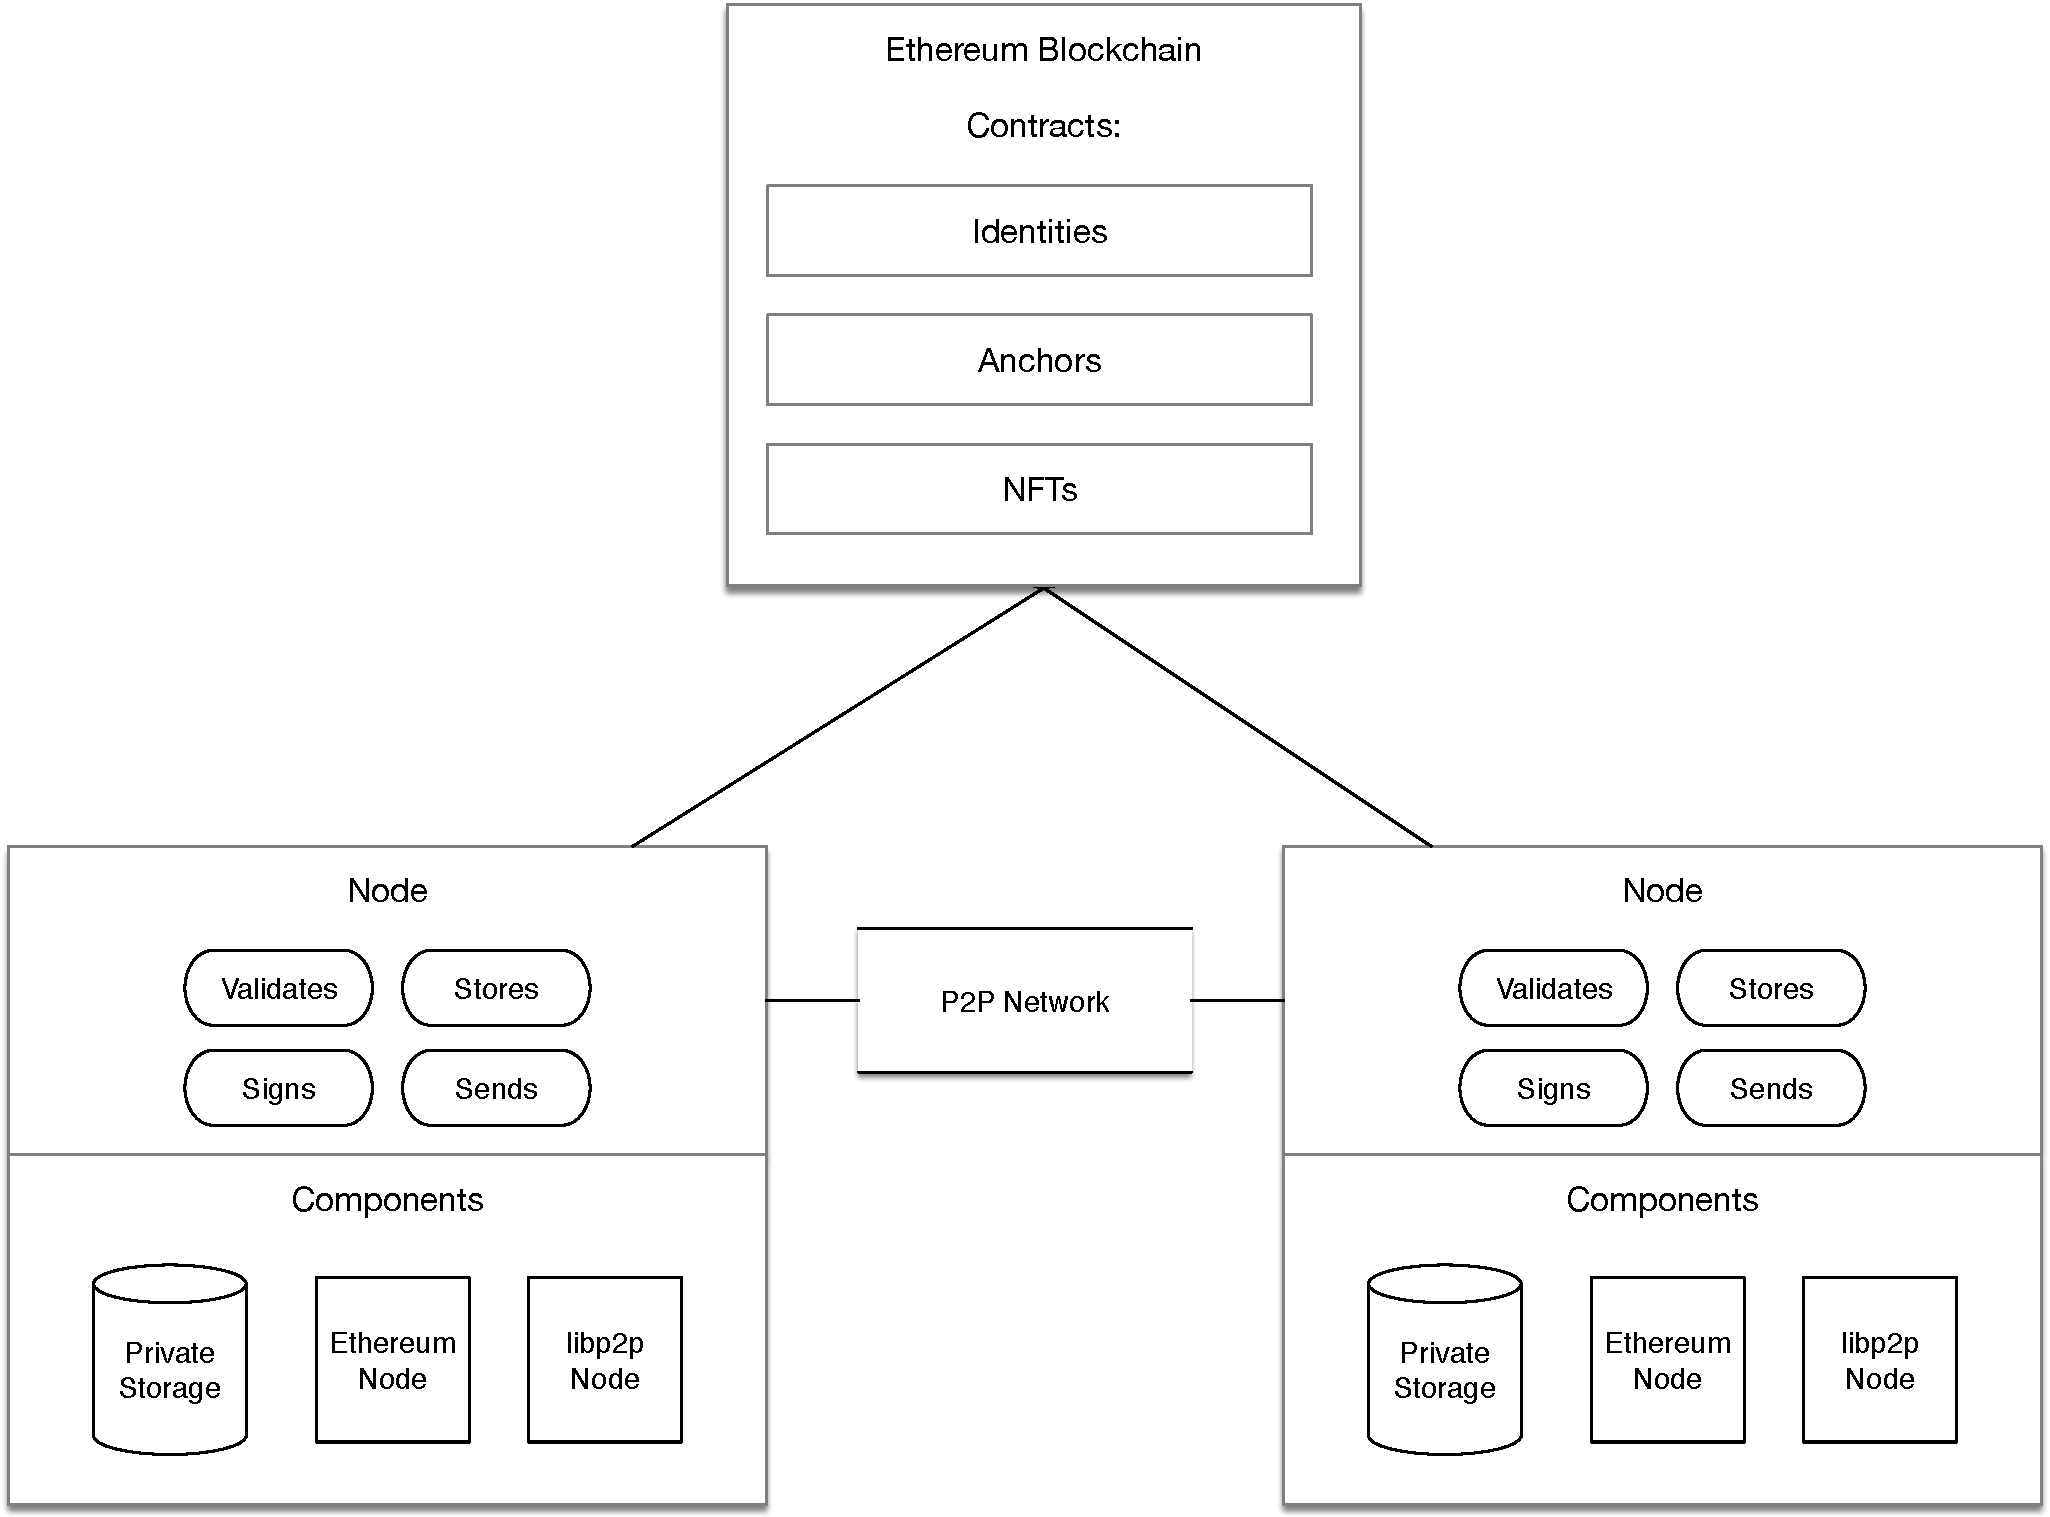
\includegraphics[width=11cm]{img/high_level_architecture.pdf}
  \caption{Overview of the components making up the Centrifuge protocol} 
  \label{fig:high_level_architecture}
\end{figure}

\subsection{Ethereum \& P2P}
Communication between nodes is done in two ways. To exchange information privately without a trusted third party or intermediary we are using libp2p' encrypted P2P communication stack. Ethereum is used as a blockchain to publish state commits to all participants, for executing smart contracts that manage identities, and allow the users to tokenize assets.

\subsection{Identity}
A node in the Centrifuge protocol uses different key pairs for signing documents and for authentication on the p2p layer. A user-deployed identity contract keeps the latest public keys. New keys can only be added by the user, and the contract can verify signatures on-chain. The identity contract thus represents the self sovereign identity of a user, as well as acting as a proxy contract for interaction with other on-chain decentralized applications. Centrifuge is adopting the DID-compatible ERC725 standard for identities.

\subsection{Documents}
A document is a well-known, structured set of fields with specific types. The protocol supports any document types as long as the formats are agreed upon and shared between the participants of a participant set-- e.g. a document can be an invoice with agreed upon fields and line items, or a purchase order. The structure of the document becomes important for reaching consensus by attaching signatures to the document state, as well as creating specific attestations about a document at a later point in time. Documents are exchanged encrypted, and are only accessible for parties involved in this private data exchange. Collaborators can be added and removed from a document. Different collaborators can update a document and publish new versions within the set of nodes with access.
A smart contract called \textit{AnchorRepository} is used for carbon dating state updates and serves as a bulletin board\cite{heiberg2018trade} to ensure that the update is made known to all collaborators. A document anchor is the root hash of the Merkle tree of the document. The tree is constructed by adding all fields of a document together with the collected digital signatures from all collaborators (an identity as defined above) as leaves in the tree. Publishing this anchor achieves that even if a party is censored on the P2P network, it can find out about the update by checking the Ethereum blockchain.
A third party can easily verify the correctness of a received document on-chain and off-chain by reconstructing the Merkle root from the document based on the well-known document structure for the respective document type. Structuring the document as a Merkle tree allows creation of proofs only revealing individual fields of the document as opposed to revealing the entire document when making a statement about it.

\subsection{NFT - Non Fungible Tokens}
An integral part of Centrifuge is interaction with other applications built on Ethereum. One way to interact with the greater ecosystem is through NFTs. Centrifuge uses privacy-enabled NFTs\cite{centrifuge2018nft} to allow for minting of NFTs that have verified attributes from private documents. The Merkle proofs that refer to a state commitment published in our \textit{AnchorRepository} contract immutably link the NFT to an off-chain document.


% TODO (Manuel): copy byte sequence definition from ethereum yellow paper
% TODO (Manuel): Define cryptographic hash function
% TODO (Lucas): we should add a section that introduces documents etc.
\section{Document and state commitments}\label{sec:doc_state_comm}

The Centrifuge protocol does not have the concept of a global state for documents. Instead, the state is only shared across collaborators of a single \textit{documents} which is the key component in the protocol.
A document has a predefined schema to represent a specific document type, like a purchase order or an invoice. A Centrifuge node can create a document and share it with others. The transport of a document happens privately over secure channels in the P2P network. Every document collaborator keeps a local copy of a document in their storage. An update of a document can be triggered by multiple collaborators and is not restricted to the initial document creator. Whenever a change is made, a
calculated merkle root of a document is committed on chain. A new version is only accepted by others if the document root hash exists in the \textit{AnchorRepository} and the set of mandatory document fields in the new version satisfy protocol-specific requirements.  A formal definition of the individual document components should expound the requirements of a valid new document state. 
\newline
\subsection{Conventions}
TODO
%\item TODO arrow notation
%\item TODO lower case in variables
%\item TODO user,identity,DID,node

Elements of $\mathbb{B}$ are an arbitrary-length byte array. $\mathbb{B}_{32}$ describes the set of 32 byte arrays. 
\textcolor{gray}{TODO:explain the used notation}.
\subsection{Document}
%---------------------------------------------------
%----- Fields
%---------------------------------------------------
\subsubsection{Fields}
\textcolor{gray}{we need to define that the schema version is defined in the coredoc}
The smallest unit of a document is called \textit{field}.  
A field $F$ is a 3-tuple  with a field name defined as $F_\texttt{name}$, a field value defined as $F_\texttt{value}$ and a salt defined as $F_\texttt{salt}$
\begin{eqnarray}
F = (F_\texttt{name},F_\texttt{value},F_\texttt{salt}) \\
\begin{array}[t]{lclclc}
F_{\texttt{name}} \in \mathbb{B} \wedge F_{\texttt{value}} \in \mathbb{B} \wedge  F_{\texttt{salt}} \in \mathbb{B}_{32} \\
\end{array}
\end{eqnarray}


\subsubsection{Document}
A document $d$  can be formally expressed as the union of the schema field set $S$ with a set of core fields called core document denoted as $C$.
\textcolor{gray}{TODO: add reference to centrifuge-protobufs}

\begin{equation}
d \equiv S \cup  C
\end{equation}
For referring to all schema fields $S$ of document or to the core document fields $C$ we introduce the following notation
\begin{eqnarray}
d_S = S \\
d_C = C
\end{eqnarray}

\subsubsection{Schema Fields}\label{sec:doc_schema_fields}
A document $d$ contains a set of fields $S$ described by a document schema. The document schema defines the type of a document. The document schema for an invoice would define the required fields for an invoice.
The set schema fields $S$ can be defined as
\begin{equation}
S = (F_{[0]},...,F_{[n]})\\
\end{equation}
In the set of specific fields $S$ for a document $d$, every field has a unique field name $F_{[i]\texttt{name}}$ to identify a member of the set.
\begin{equation}
F_{[i]} \in  S \Rightarrow F_{[i]\texttt{name}} \neq  F_{[j]\texttt{name}} \, ; \forall F_{[j]}  \in S, i \neq j 
\end{equation}
%\begin{equation}
%\{x \in \{0..n\}| \nexist y \in \{0..n\}\x: F[x]_i=F[y]_i \land x & \neg & y \}
%\end{equation}

\subsubsection{Core Document Fields\label{Core Document}}\label{sec:doc_core_doc_fields}
The core document $C$ defines the required fields for every document $d$.
The core document contains signatures, hashes, and other relevant information that allows users to exchange any document data.
 
We introduce the fields in $C$ step by step in the following section and define the required constraints of the core document fields. Variables denoted with $R_{\texttt{x}}$  are not part of the core document but are calculated based on core document fields. $R_{\texttt{x}}$ variables are needed for signing and for anchoring documents in the smart contract. A document field which is a core document field is denoted with $d_{\texttt{x}}$. 
The core document\footnote{\url{https://github.com/centrifuge/centrifuge-protobufs/blob/master/coredocument/coredocument.proto}} includes other fields not mentioned in this section which are introduced in the following sections step by step.
\begin{description} 
\item{\textbf{Identifier}} a $\mathbb{B}_{32}$ value defines the unique identifier of a document, formally $d_{\texttt{id}}$ 
\item{\textbf{Current Version}} a $\mathbb{B}_{32}$ value defines a unique id for the current version of a document, formally as $d_{\texttt{current}}$
\item{\textbf{Previous Version}} a $\mathbb{B}_{32}$ value needed to refer to the previous version of a document, formally as $d_{\texttt{prev}}$
\item{\textbf{Next Version Pre Image}} is a $\mathbb{B}_{32}$ value needed to define the next version of a document,  formally as $d_{\texttt{next-img}}$
\item{\textbf{Next Version}} a $\mathbb{B}_{32}$ value defines a unique identifier for the next version of a document, formally $d_{\texttt{next}}$
\item{\textbf{Document Root}} a $\mathbb{B}_{32}$ value defines a root hash for document, formally $R_{\texttt{doc-root}}$
\item{\textbf{Signing Root}} a $\mathbb{B}_{32}$ value defines the root hash of the Merkle tree containing all fields except for the signatures, formally $R_{\texttt{signing}}$
\item{\textbf{Signatures}} a set of signatures of the signing root denoted as $d_{\texttt{signatures}}$
\item{\textbf{Previous Root}} a $\mathbb{B}_{32}$ value defines the document hash of the previous version of the document. The previous root denoted as $d_{\texttt{prev-root}}$
\end{description}


%---------------------------------------------------
%----- Version History
%---------------------------------------------------
\subsubsection{Version History}\label{sec:version_history}
The version history $H$ is a set of documents. An update of an existing document in the Centrifuge protocol happens by creating a new version and linking this new version to the previously existing version. 
We define the set of all documents as $D$:
\begin{equation}
d \in D
\end{equation}
Every node keeps a history of all versions of a document in which they are listed as a collaborator.
\begin{equation}
H = (d_{[0]},...,d_{[n]})
\end{equation}
\newline
In the initial version of a document $d_0$, the current version and the identifier will be equal.
\begin{equation}
d_{[0]{\texttt{id}}} = d_{[0]\texttt{current}}
\end{equation}
\newline
The fields for the previous document root hash $D_{\texttt{prev-root}}$ and for the $D_{\texttt{prev}}$ id will be empty in the initial version.
\begin{eqnarray}
d_{[0]{\texttt{prev-root}}}& = & \emptyset \\
d_{[0]{\texttt{prev}}} & = & \emptyset
\end{eqnarray}
\newline
For all other documents $D$ in a version history $H$, the following conditions must be true:
\newline
\newline
Every document in a version history $H$ must have the same identifier.
\begin{equation}
\{d_{[i]} \in H \mid \forall d_{[j]} \in H :d_{[i]\texttt{id}} = d_{[j]\texttt{id}} \}
\end{equation}
\newline
The current version field of a document must be equal to the next version field of the previous document.
\begin{equation}
d_{[i]\texttt{current}} = d_{[i-1]\texttt{next}} 
\end{equation}
\newline
The previous version field of a document must be equal to the current version field of the predecessor document.
\begin{equation}
d_{[i]\texttt{prev}} = d_{[i-1]\texttt{current}} 
\end{equation}
\newline
The previous root hash of a document must be equal to the document root hash of the predecessor document.
\begin{equation}
d_{[i]\texttt{prev-root}} = d_{[i-1]\texttt{doc-root}}
\end{equation}
\newline
The current pre-image of a document must be equal to the next pre image of the predecessor document.
\begin{equation}
d_{[i]\texttt{current-img}} = d_{[i-1]\texttt{next-img}}
\end{equation}
\newline
The history of the document can therefore be seen as a doubly linked list. Every document has the document hash $d_{\texttt{previous}}$ of the predecessor document and defines the $d_{\texttt{id}}$ of the next one.\\\\
A node which performs a document update defines the the next version identifier $d_{\texttt{next}}$.
\begin{equation}
d_{[i]\texttt{next-img}} = \texttt{RAND(32)}
\end{equation}
\begin{equation}
d_{[i]\texttt{next}} = \mathtt{sha256}(d_{[i]\texttt{next-img}})
\end{equation}
\newline
The field $d_{\texttt{next-img}}$ is needed to prevent malicious anchoring of documents by non-collaborators. The value therefore must be kept secret from any non-collaborators. The function $\texttt{RAND(32)}$ is a cryptographically secure random function and returns a byte 32 array. The function $\mathtt{sha256}$ denotes hash function SHA-2 256. 

By referencing the previous root each state $d$, the history becomes an immutable attribute committed to in each version. To traverse the history $H$, one can follow the $d_{\mathtt{prev-root}}$ and $d_{\mathtt{prev}}$. To move forward in the list of history, $H$, one can go from $d_{\mathtt{next}}$ to $d_{\mathtt{current}}$.
\begin{figure}[thpb]
  \centering
  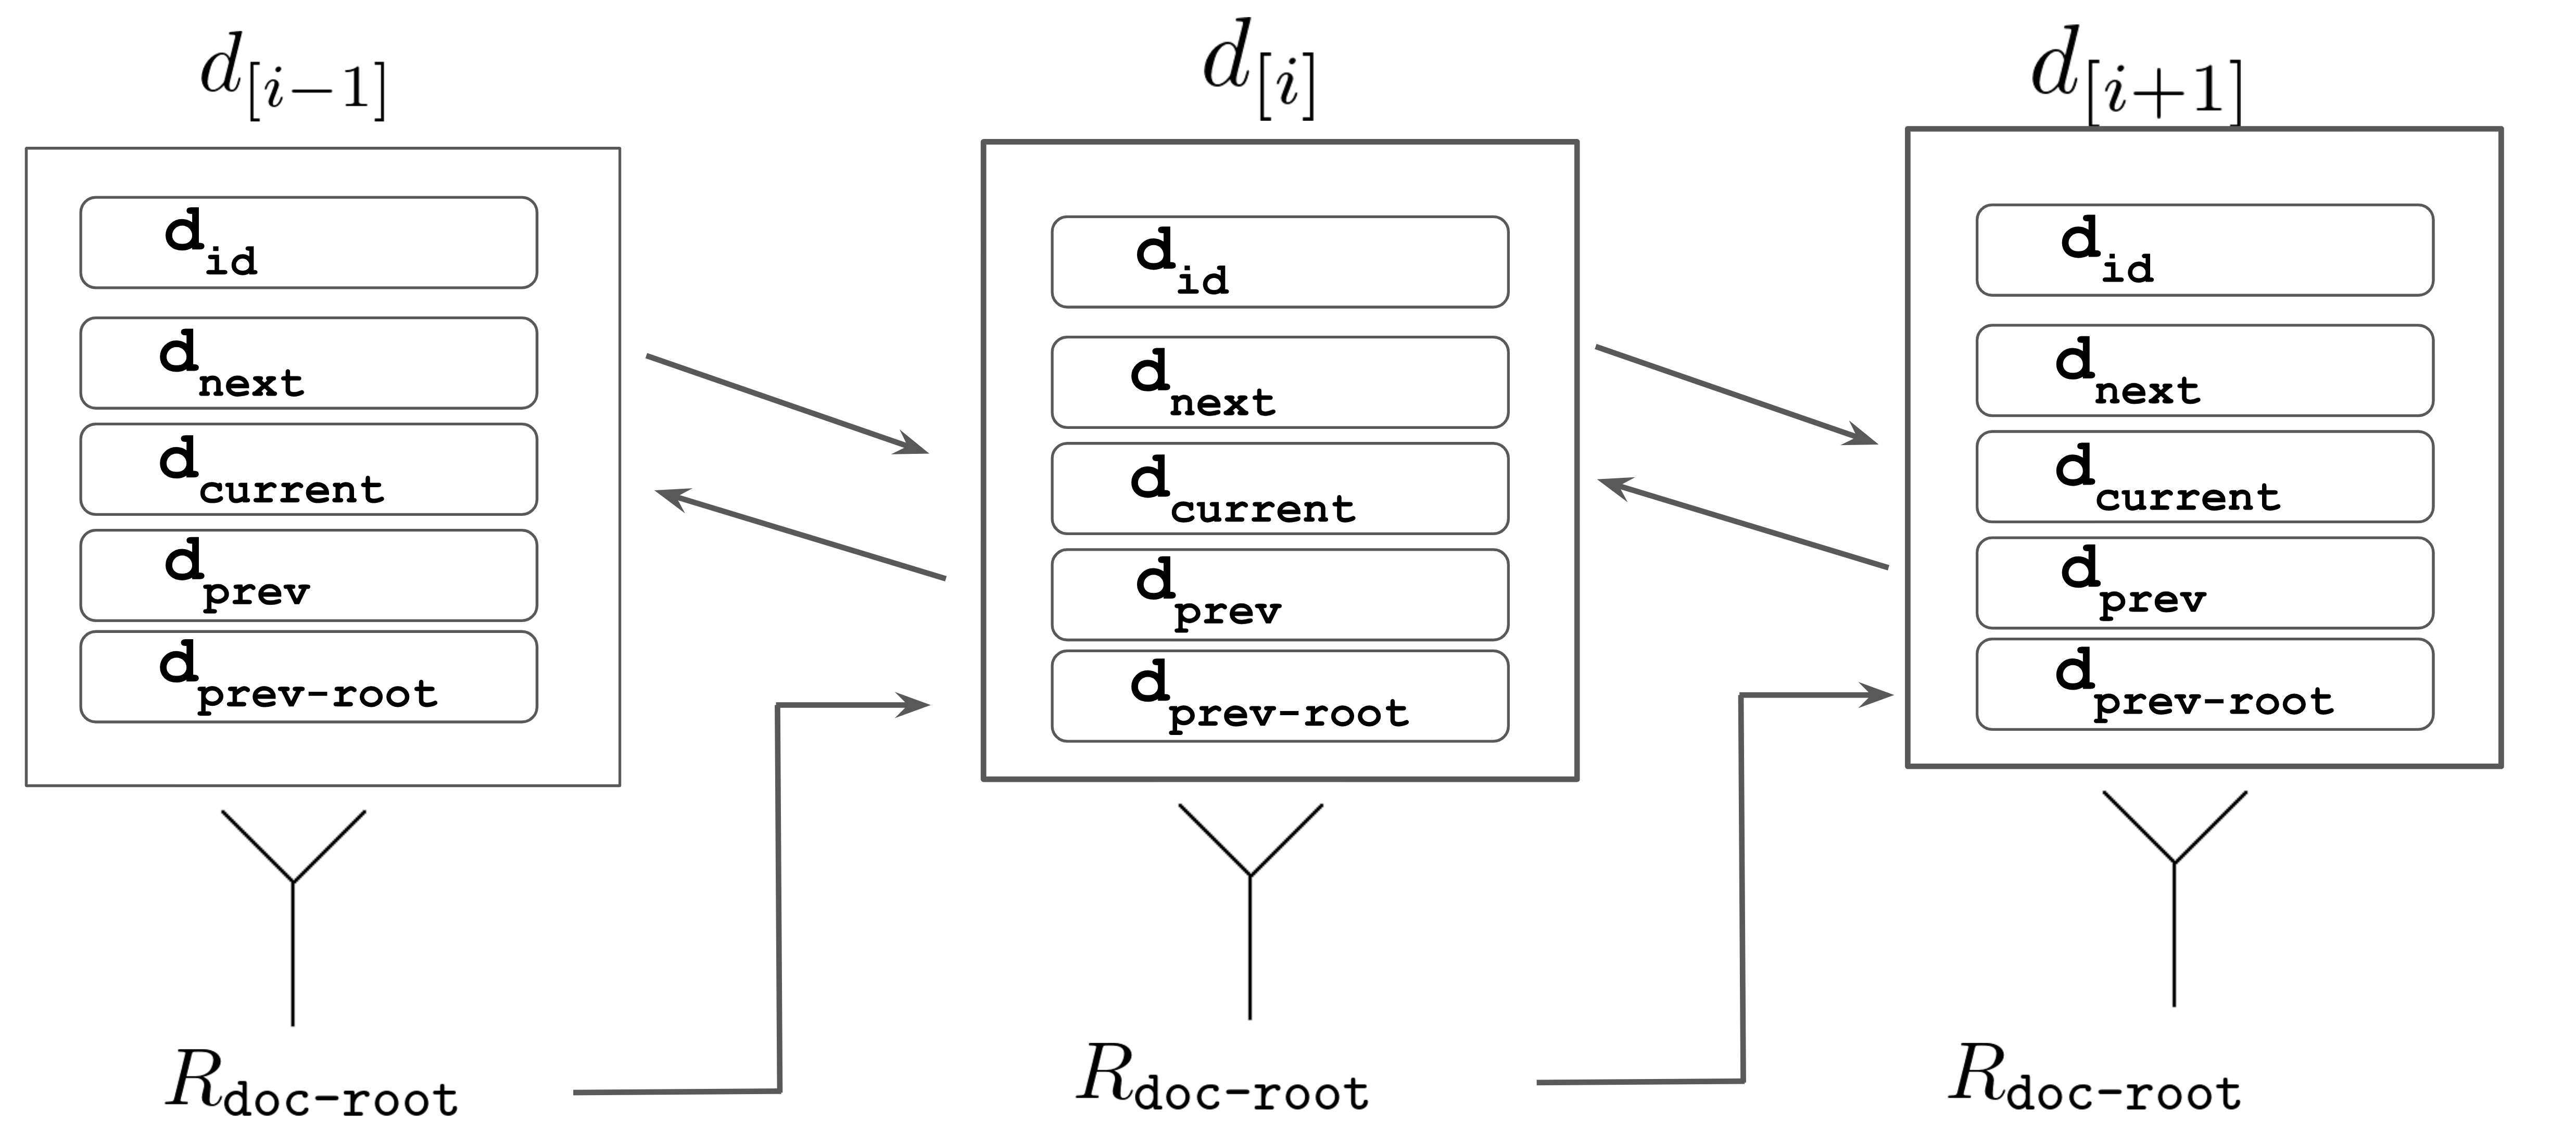
\includegraphics[width=16cm]{img/documents-history-v2.png}
  \caption{Doubly linked list of different versions of a document. Indicating the relationship between different document index fields. The document root $R_{\texttt{doc-root}}$ is stored in the anchor registry and not in the document itself.} 
  \label{fig:documents}
\end{figure}


%---------------------------------------------------
%----- Calculation of the Root Hashes
%---------------------------------------------------
\subsection{Calculation of the Root Hashes}
Every root hash of a document $R_{\texttt{doc-root}}$ is stored in the
\textit{AnchorRepository} smart contract. The document root hash is calculated from three different Merkle trees (see Fig. \ref{fig:root-hash}). 
\subsubsection{Merkle Tree of Fields}
A Merkle tree is a way to calculate a unique hash from a set of items. We formally define a Merkle tree function $\mathcal{M}$ to calculate a root hash $R \in \mathbb{B}_{32}$ of document fields $F$. The implementation of the Merkle tree function is introduced in Sec. \ref{sec:precise_proofs}.
 \begin{eqnarray}
 R & = &\mathcal{M}(F_{[0]},...,F_{[n]}) \\
 R & \in & \mathbb{B}_{32}
\end{eqnarray}
\newline
\subsubsection{Schema Root and CoreDocument Root}
As a first step, we calculate the Merkle root of the schema fields $S$ and the core document fields $C$ of a document $d$\\\\
\textbf{Schema Root} The Merkle root of the document schema data, formally $R_{{\texttt{schema}}}$ 
\newline
\begin{equation}
    R_{{\texttt{schema}}} = \mathcal{M}(d_S)
\end{equation}
\newline
\textbf{CoreDocument Root} the Merkle root of the core document data, formally $R_{{\texttt{core}}}$ \\
\begin{equation}
R_\texttt{core} = \mathcal{M}(d_C)\\
\end{equation}
 \subsubsection{Signing Root}
The $R_{\texttt{signing}}$ is calculated from the SHA256 hash of the concatenated $R_\texttt{core}$ and $R_{\texttt{schema}}$
\newline
\begin{equation}
R_{\texttt{signing}} = \texttt{sha256}(R_\texttt{core}\| R_{\texttt{schema}})
\end{equation}\\
We formally define a helper function for calculating the $R_{\texttt{signing}}$ 
\begin{eqnarray}
R_{\texttt{signing}}& =&\mathsf{calculateSigningRoot}(d) \\
\mathsf{calculateSigningRoot}(d)& =& \texttt{sha256}(\mathcal{M}(d_C)\| \mathcal{M}(d_S))
\end{eqnarray}
 \subsubsection{Signatures Root}
 A Merkle root of the collaborator signature must be part of the document root hash $R_{\texttt{doc-root}}$. The signatures are relevant for the document consensus, explained in the following chapters. \\\\
\textbf{Signature Root} A signature root hash defines the Merkle root of all signatures $d_{\texttt{signatures}}$, formally $R_{\texttt{signatures}}$:
\newline
\begin{equation}
R_{\texttt{signatures}} = \mathcal{M}(d_{\texttt{signatures}})\\
\end{equation}
 \subsubsection{Document Root}
The final  document root hash $R_{\texttt{doc-root}}$ of the entire document $d$ is defined as the SHA256 hash of the concatenated signing root hash $R_{\texttt{signing}}$ and signature root hash $R_{\texttt{signatures}}$ 
\newline
 \begin{equation}
R_{\texttt{doc-root}} =  \texttt{sha256}(R_{\texttt{signing}}\|R_{\texttt{signatures}})
\end{equation}\\
A tree of the  $R_{\texttt{doc-root}}$ calculation. (see Fig. \ref{fig:root-hash})

%TODO (Manuel): Why sometimes R and D?

%All information related to the document is stored in a structured protobuf message called CoreDocument, \mathsf{CD}, along with a document-specific message, Data, \mathsf{D} such as an Invoice or PurchaseOrder. Both messages are serialized with precise proofs into \\mathsf{CD} 

\begin{figure}[thpb]
\centering
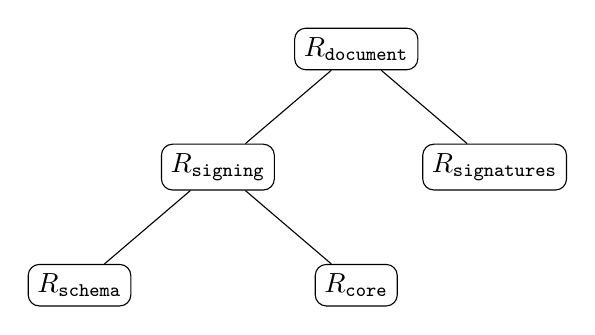
\begin{tikzpicture}[sibling distance=10em,
  every node/.style = {shape=rectangle, rounded corners,
    draw, align=center, %top color=white, bottom color=gray!20
    }]]
  \node {$R_{{\texttt{document}}}$}
    child { node {$R_{{\texttt{signing}}}$}  child { node {$R_{{\texttt{schema}}}$}  
    } child { node {$R_{{\texttt{core}}}$}
    } }
    child { node {$R_{{\texttt{signatures}}}$}};
\end{tikzpicture}
\caption{Calculation of the last layers of the document merkle tree. The leafs are the roots of merkle trees from the different document parts }\label{fig:root-hash}
\end{figure}
We can define a second help function called $\mathsf{calculateDocumentRoot}(d)$ for calculating the entire $R_{\texttt{doc-root}}$. 
\begin{eqnarray}
R_{\texttt{doc-root}}& =&\mathsf{calculateDocumentRoot}(d) \\
\mathsf{calculateDocumentRoot}(d)& = & \texttt{sha256}( \mathsf{R_{\texttt{signing}}}\| \mathcal{M}_{\texttt{tree}}(d_S))
\end{eqnarray}
% describe how a document root hash is calculated
%---------------------------------------------------
%----- State Commitment
%---------------------------------------------------
\subsection{State commitment}

\subsubsection{Anchors}
An anchor is the root hash of a document $R_{\texttt{doc-root}}$ stored in an Ethereum smart contract called \textit{AnchorRepository}. 
\\\\
Every new document version $d'$ must commit its  document root hash $R_{\texttt{doc-root}}$ to the registry. A new document $d'$ is only valid and accepted if the $R_{\texttt{doc-root}}$ exists as an anchor in the registry.\\
%\textcolor{gray}{TODO: introduce blockheight}
\begin{eqnarray}
A &=& (A_{\texttt{anchor-id}}, A_{\texttt{anchor-root}}, A_{\texttt{anchor-blockheight}})\\
A_{\texttt{anchor-id}} & = & d_{\texttt{current}} \\
A_{\texttt{anchor-root}} & = & R_{\texttt{doc-root}} \\
A_{\texttt{anchor-blockheight}} & = & \texttt{block.number}
\end{eqnarray}
\\
The anchor id of a new document $d_{[i]{\texttt{current}}}$ is defined by the previous document $d_{[i-1]\texttt{next-img}}$. The same image is stored in the current 
document in $d_{[i]\texttt{current-img}}$. The hash of the $d_{[i]\texttt{current-img}}$ defines the current document identifier and the anchor id.
\begin{eqnarray}
d_{[i]\texttt{current}}& = & \mathtt{sha256}(d_{[i-1]\texttt{next-img}})\\
A_{\texttt{anchor-id}}& = & d_{[i]\texttt{current}}
\end{eqnarray}
The \texttt{block.number} contains the Ethereum block number the transaction got mined and acts as a timestamp for the anchor.
\subsubsection{Verifying a document}
Any user can verify the correctness of the document by comparing the root hash to the committed hash on chain. We formally define a method called $\mathsf{getAnchor}$ which returns an anchor from the contract.
\begin{eqnarray}
A_{\texttt{anchor-current}} & \xleftarrow[]{\text{ETH}}& \mathsf{getAnchor}(d_{[i]{\texttt{current}}}) \\
A_{\texttt{anchor-next}} & \xleftarrow[]{\text{ETH}} & \mathsf{getAnchor}(d_{[i]{\texttt{next}}}) \\
\end{eqnarray}

\subsubsection{Latest Version}
Because in each document (state) update the next anchor id is already defined, anyone can verify that they have the latest version by checking the anchor registry. A document $d_{[i]}$ is the latest version if the following condition is true:
\begin{equation}
A_{\mathtt{anchor-current}} = R_{\mathtt{doc-root}} \quad \wedge \quad A_{\mathtt{anchor-next}} = 0
\end{equation}
If an anchor for $A_{\mathtt{anchor-next}}$ exists, the current document $d_{[i]}$ is not the latest version. It is not possible to overwrite an existing anchor id or invalid it. For committing an anchor the $d_{[i]\texttt{current-img}}$ is needed therefore only document collaborators could propose a next version.

\subsubsection{Pre-Commit}
A document is committed only after reaching consensus with the other collaborators on the document. Consensus is reached by getting a cryptographic signature from other parties by sending them the signing root. To deny the counter-party the free option of publishing its own state commitment upon receiving a request for signature, the node can first publish a pre-commit.
A pre-commit locks a commit to a specific document state for a given anchor id for a predetermined number of blocks. Only the \texttt{msg.sender} of the pre-commit is allowed to commit a corresponding anchor before the pre-commit has expired.

\begin{equation}\\
    \mathsf{preCommit}(d_{[i]\texttt{current}},R_{\texttt{signing}}) \xrightarrow[]{\text{ETH}} \mathsf{AnchorRepository}
    %TODO: leftover? M_{\texttt{proof}}(R_{\texttt{doc-root}})
\end{equation}\\
The pre-commit stores the provided signing root $R_{\texttt{signing}}$ on the smart contract. Only a $R_{\texttt{doc-root}}$ in the commit which includes the same $R_{\texttt{signing}}$ is accepted as a valid commit. 
It is not possible to provide a new preCommit $R_{\texttt{signing}}$ within the next  blocks for the given anchorId.\\
In the event that the user does not provide a commit within the lock time, the commit will be unlocked, and the \texttt{preCommit} method will be open to everyone again.

\subsubsection{Commit}
The anchor registry's \texttt{commit} method does not have any restrictions, except for the pre-commit flow as described above. If no valid pre-commit exists, anyone can commit an anchor to the registry. A commit of a new anchor is described by the following function. 
\begin{equation}\\
    \mathsf{commit}(d_{[i]\texttt{current-img}},R_{\texttt{doc-root}},P_{\texttt{sign-proof}}) \xrightarrow[]{\text{ETH}} \mathsf{AnchorRepository}
    %M_{\texttt{proof}}(R_{\texttt{doc-root}})
\end{equation}\\
\textbf{Next Pre-Image }\\
The commit method hashes $d_{[i−1]\texttt{next-img}}$ inside the smart contract to get the $A_{\texttt{anchor-id}}$. The $d_{[i−1]\texttt{next-img}}$ of the previous version is needed to commit the next version. It is not possible to use $d_{[i−1]\texttt{next}}$ (equal to $d_{[i]\texttt{current}}$) directly. In some cases, the field  $d_{\texttt{next}}$ is revealed to the outside world to prove the latest version of a document. (See \ref{sec:nft}). The anchor contract challenges the submitter to reveal the pre-image to avoid an attacker committing an malicious anchor for $d_{\texttt{next}}$. The field $d_{\texttt{next-img}}$ is never revealed to the outside world. \\
\\
\textbf{Signing Root Proof }\\
In case a pre-commit exists for the \texttt{anchorId}, calculated by hashing the given pre-image, the \texttt{msg.sender} must be the same as in the pre-commit. In the pre-commit, the signing-root $R_{\texttt{signing}}$ has been stored. A merkle proof verifies if the $R_{\texttt{signing}}$ is part of the $R_{\texttt{doc-root}}$ tree. $P_{\texttt{sign-proof}}$ is an array of $\mathbb{B}_{32}$ arrays which contains the needed sibling hashes for the merkle proof. 


%TODO
%\begin{eqnarray}
%\mathsf{commit}(d_{[i-1]\texttt{next-img}},R_{\texttt{doc-root}}) \\
%\mathsf{getAnchor}(d_{[i]{\texttt{current}}}) \to A_{\texttt{anchor}} \\
%\mathsf{getAnchor}(d_{[i]{\texttt{next}}}) \to A_{\texttt{anchor-next}} \\
%\sigma_{t+1} = T(\sigma_{t},d_{[i]},A_{\texttt{anchor}},A_{\texttt{anchor-next}})
%\end{eqnarray}



%\subsubsection{Commit old version}
%A node can commit to a state by publishing the root hash of the document on a contract. The document has a 32 byte randomly generated identifier, $I$ under which the commitment \math{c} is published. 

%TODO (Manuel): C used for something other than the C above (CoreDoc Fields)


%\begin{equation}
%c = C(I, RH(D)
%\end{equation}

%The state commitment function is a transaction on the Ethereum \texttt{AnchorRepository} contract\footnote{https://github.com/centrifuge/centrifuge-ethereum-contracts/blob/develop/contracts/AnchorRepository.sol}. It has a list of previous commitments and allows addition but not modification of commitments. We call these commitments \textit{anchors}.

 

\subsection{Protobuf for Schema Definitions}\label{sec:protobuf_schema}
%TODO (Lucas): finish precise proofs 
Every document has a predefined schema which is agreed upon by all network participants. The Protobuf\footnote{\url{https://developers.google.com/protocol-buffers/}} message format is used for defining the document schema. It was chosen as a schema and serialization standard for its efficient binary format, broad support in different programming languages and fixed schema. An example of such a message is shown below in Fig. \ref{fig:example_document}. 

\begin{figure}[ht]
  \caption{An example protobuf definition}
  \label{fig:example_document}
  \begin{lstlisting}
  message ExampleDocument {
    string name = 1;
    repeated int numbers = 2;
  }\end{lstlisting}
\end{figure}

All documents that are supported by Centrifuge protocol are hosted on GitHub in a repository at \url{https://github.com/centrifuge/centrifuge-protobufs}.  

%TODO: write how CoreDocument has an include any.Any{} and that this is how the type is defined and add it as a field. mention that this structure was chosen because of a tradeoff in protobufs


\subsection{Precise proofs: Merkle tree format}\label{sec:precise_proofs}
Merkle trees are efficient ways to prove membership in a set. By encoding the leaves of the tree, a Merkle tree can be used to make a proof about the value of a field specific in the schema. The value of the field is prefixed with a byte encoded field path, $P$, and a salt, $S$. 


\subsubsection{Path encoding}
The reference for the path encoding is the precise-proofs\footnote{\url{https://github.com/centrifuge/precise-proofs}} library but is briefly summarized here. Protobuf uses 32bit unsigned integers to identify fields within a message uniquely. The property $p$ is defined using these values. The encoding of property names also supports nested messages, mappings, as well as repeated fields (arrays). 
\begin{equation}
    p_{F} = \mathsf{FieldToProperty}(F_{\texttt{name}})
\end{equation}

\begin{figure}[ht]
  \centering
  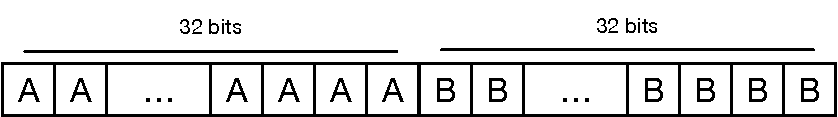
\includegraphics[width=11cm]{img/property_bits.pdf}
  \caption{The field numbers for a path \texttt{"A.B"} are concatenated into a fixed length delimited byte value} 
  \label{img:property_bits}
\end{figure}

In this paper, we refer to the fields by their human readable name using JavaScript-style dot notation for easier readability. However, the byte format will be used when encoding a leaves.


\subsubsection{Salts}
When proving, the hash of the sibling of the field is revealed. A salt is therefore added to the value of the leaves in order to avoid a rainbow table attack on sibling leaves revealed in a proof. The salt $F_{\mathsf{salt}}$ is stored in a special field on the \textit{CoreDocument} protobuf message called \texttt{salt} in form of a map where a salt is stored for each field by the property $p_F$.

\subsubsection{Construction of the tree}
For each leaf, $\lambda$, the name $P$, the salt $S$ and the value $v$ are appended and then hashed with $\mathtt{sha256}$.

\begin{eqnarray}
\lambda = \mathtt{sha256}(p_{F} \parallel F_{\texttt{value}} \parallel	 F_{\texttt{salt}})\\
\mathrm{T}(\mathrm{D}) = \mathcal{M}({\lambda_{1} \parallel \lambda_{2} \parallel ... \parallel \lambda_{n}})
\end{eqnarray}

\subsubsection{Merkle Proof Validation}\label{sec:merkle_proof_validation}
A Merkle proof can be seen as a function which proves if a provided field $P_\mathtt{field}$ is part of document. By calling the NFT mint method the value of these fields is revealed to the public. 
\begin{equation}
\begin{split}
v = \mathcal{M}_{\texttt{proof}}(A_{\texttt{anchor-current}},P_\mathtt{field},P_\mathtt{sibling-hashes}) \\
v \in \{0;1\}
\end{split}
\end{equation}
The $P_\mathtt{field}$  could be any field of the core document $d_C$ or the schema field $d_S$. The required $P_\mathtt{sibling-hashes}$ can be generated with the precise proofs library inside the node and contains the siblings of the field in each layer of the Merkle tree.  
\section{Participants}\label{sec:particpiants}
A user of Centrifuge is defined as an entity that owns a set of keypairs and is running a node to communicate with other nodes and the smart contracts. A user can be an individual or a different entity. Digital signatures are used to authenticate a user. A user controls a smart contract on Ethereum where they publish the public keys in use.

\subsection{Self-Sovereign Identity}\label{sec:identity_contract}
A W3C standard for self-sovereign identities called DID (Decentralized Identifiers)\cite{Decentra50:online} is currently under development. Centrifuge identities are compatible with the ERC725 standard (see below \ref{sec:erc725}) for identities which is self-sovereign (SSI), as well as DID compatible.

%TODO: maybe mention Meta transaction which are currently not included in the standard
\subsubsection{ERC725 Identity Standard}\label{sec:erc725}
Many decentralized applications built on Ethereum require a form of identity to standardize interactions. A set of different standards for identities have been proposed to address these standardization issues\cite{EIPseip791:online}\cite{ERCLight27:online}. In ERC725\footnote{A newer version of ERC734 dated February 2019 defines key management, while the newer ERC725 v2 defines only the proxy functionality. The Centrifuge protocol currently implements ERC725 v1.}, a user's identity is represented as a smart contract. The user is the owner of the identity, and retains exclusive control over who is allowed to add new keys and interact with other contracts in Ethereum on behalf of the identity. Centrifuge is adopting the ERC725 standard but we are fully aware it might in change in the future and the current version is not final.
\subsubsection{DID - Centrifuge ID}\label{did}
The address of the identity contract represents the unique ID of a user in the protocol. The ID can be extended with information about the Ethereum network to represent a valid DID. A sample DID representation of an identity address\cite{rwot6san30:online}:
\begin{quote}\texttt{did:erc725:mainnet:2F2B37C890824242Cb9B0FE5614fA2221B79901E}\end{quote}
Within Centrifuge, only the address of the identity contract is used to describe a user ID as the only supported identities are Ethereum smart contracts.
\begin{equation}
        \mathtt{DID} \in \mathbb{B}_{20}
\end{equation}
\subsubsection{Key Management}
A user can add different public keys to their identity. A number of different signature and encryption standards are supported. A key can be seen as a 4-tuple.
\begin{equation}
K = (K_\mathtt{public},K_\mathtt{private},K_\mathtt{type},K_\mathtt{purpose})\\
\end{equation}
An ERC725 key is a 3-tuple of three elements, not including the private key of the user. A user can use the same key for multiple purposes and needs only to add it once to the identity contract.
\begin{eqnarray}
K_\mathtt{ERC725} & = & (K_\mathtt{public},K_\mathtt{type},K_\mathtt{purposes})\\
K_\mathtt{public} & \in & \mathbb{B}_{32} \\
K_\mathtt{type} & \in & \mathbb{B}_{32} \\
 K_\mathtt{purposes} &\in & \mathbb{B}_{32}^n \\
  |K_\mathtt{purposes}| & >  & 0
\end{eqnarray}
The $K_\texttt{ERC725}$ key is the representation of a $K$ in the identity contract. 
%TODO Manuel: at least one purpose is required
\subsubsection{Identity}
Users have an unique id $I_\mathtt{DID}$ which is the address of their identity contract. A user needs at least 4 different keys for purposes needed in the protocol.It is possible to add other keys to the identity contract or to add keys with same purpose. 

We can formally define the identity of a user as:
\begin{eqnarray}
    I& = &(\mathtt{DID},k_\mathtt{man},k_\mathtt{p2p},k_\mathtt{sign},k_\mathtt{action}) \\
    k & \in & K
\end{eqnarray}


\subsubsection{Proxy Contract}
A contract in Ethereum does not differentiate between calls from a user account or another contract. A proxy contract is a contract that can forward a call to another contract. From the perspective of the called contract, the \texttt{msg.sender} is the proxy contract. Identities act as a proxy contract. This allows an identity contract to interact with other contracts like any other account. The identity owner can add Ethereum addresses with the purpose \texttt{ACTION-KEY} to their identity that are able to invoke such proxy calls. 

\begin{figure}[thpb]
  \centering
  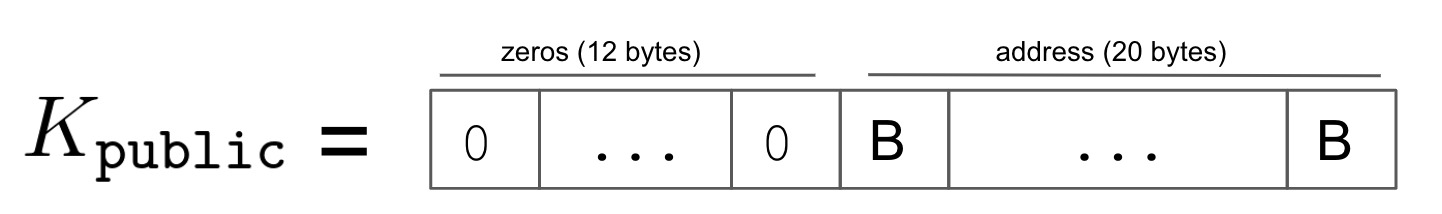
\includegraphics[width=10cm]{img/address.png}
  \caption{Storage of an Ethereum address in the identity contract.} 
  \label{fig:address}
\end{figure}
These Ethereum addresses are allowed to use the proxy functionality of the contract. Later, the owner can revoke the permissions if needed. An Ethereum address has 20 bytes $\mathbb{B}_{20}$. The $K_\texttt{public}$ requires the public key to be 32 bytes. An Ethereum address needs to be converted into a 32 bytes array by adding 12 leading zeros to it. (see figure \ref{fig:address})

\subsubsection{Key Types}\label{sec:key_types}
In the protocol, four different key types are required. (see \ref{tab:keys}) The identity contract defines a set of methods for adding and revoking keys.  Every public key must be added to the identity contract. The ERC725 standard defines a set of pre-defined key purposes. It is possible to add individual purposes for the Centrifuge protocol.
\begin{table}[!htbp]
\label{tab:keys}%TODO: proper reference above
\centering
\begin{tabular}{|l|l|l|}
\hline
 \textbf{Purpose}       & \textbf{Purpose ID} & \textbf{Key Type} \\ \hline
Management Key &      1      &          secp256k1 \\ \hline
Action Key    &      2      &            secp256k1     \\ \hline
Centrifuge Signing Key   &       \texttt{SIGNING} = $\mathtt{sha256}$(\texttt{"CENTRIFUGE@SIGNING"})     &            secp256k1    \\ \hline
Centrifuge P2P Discovery &    \texttt{P2P\_DISCOVERY} = $\mathtt{sha256}$(\texttt{"CENTRIFUGE@P2P\_DISCOVERY"})         &            ED25519 \\ \hline
\end{tabular}
\caption{Overview of the key types used in the Centrifuge protocol.}
\end{table}
% TODO: proper quotation marks in above table

\subsubsection{Management Key}
The management key, $k_\mathtt{man}$, is a reserved key type in the ERC725 standard and represents the key pair of the owner. This key has the right to add new keys, revoke existing ones, or allow other addresses to use the proxy functionality.
\subsubsection{Action Key} 
The action key, $k_\mathtt{action}$, is a reserved key type in the ERC725 standard. An action key can be added by a management key and allows the owner of the action key to use the proxy functionality.  Only an Ethereum address stored as a key with the action purpose can trigger the proxy functionality. \\
\subsubsection{Centrifuge Signing Key}
The signing key, $k_\mathtt{sign}$, is a Centrifuge specific key purpose. It is used to sign documents together with other collaborators. The key type needs to be secp256k1 because a signature can be part of a Merkle proof and needs to be verified on-chain to guarantee another identity has signed a document. The identity contract has a method which verifies signatures based on a key purposes. Secp256k1 signature verification has native support in the EVM.
\subsubsection{Centrifuge P2P Discovery Key}
See section \ref{did-node}.
\subsubsection{Deployment of an Identity}
An identity contract is deployed by a user through a well-known, Centrifuge-specific Factory contract, the  \texttt{IdentityFactory} contract, that constructs the identity for the caller and keeps track of identities which are created within the Centrifuge network. This tracking allows for later verification of identity "validity" for users within the network.
%TODO Manuel
\subsubsection{Revoking Keys}
The ERC725 identity standard allows key revocation. A revoked key is not removed from the identity contract.  Currently other Centrifuge contracts like the NFT registry only supporting ERC725 identity contracts created by the Factory contract. In our ERC725 version the key is only marked as revoked. In the protocol, a message which is signed with a revoked key before the key was revoked is accepted. However, a message which is signed with a revoked key after the key was revoked is not accepted.
%TODO add graphic for better understanding







\section{Document State Consensus}
\label{sec:consensus}
In \ref{sec:doc_state_comm}, we introduced how state is committed to and in \ref{sec:particpiants}, we defined the attributes and behaviors of individual actors in the system. Building upon this, we now introduce our mechanism for enabling the reaching of consensus among different parties.
\subsection{Consensus Trade-offs}
For the initial protocol version we have decided to avoid a fully BFT consensus scheme. The protocol does not guarantee data availability for every participant. Instead, the focus is on preserving privacy in the optimistic case and requiring any consensus failures to be settled out of band. 

\subsection{Roles and Rules}\label{sec:roles_rules}
A document has a set of roles, $d_{\mathtt{roles}}$ and rules, $d_{\mathtt{rules}}$ that can be attached to a role. Nodes have particular roles, and the rules give them certain capabilities. They are listed in the set of $Role_{\mathtt{members}}$.

\begin{eqnarray}
Role &= &(Role_\mathtt{id},Role_{\mathtt{members}}) \\
Role_{\mathtt{id}} &\in & \mathbb{B}_{32}\\
Role_{\mathtt{members}}  &=& (Member_{[0]},...,Member_{[n]}) \\
Member &\in & \{\mathtt{DID};\mathtt{access\_token};\mathtt{NFT}\} \\
d_{\mathtt{roles}} & = & (Role_{[0]}, ..., Role_{[n]})
\end{eqnarray}

%\begin{eqnarray}
%    Role & \equiv & (Role_{\mathtt{id}}, Role_{\mathtt{members}}, Role_{\mathtt{nfts}}) \\
 %   Role_{id} & \in & \mathbb{B}_{32} \\
  %  Role_{\mathtt{members}} & \equiv &  (\mathtt{DID}_0, %..., \mathtt{DID}_n)\\
  %  d_{\mathtt{roles}} & \equiv & (Role_1, ..., Role_n) \\
%\end{eqnarray}

\begin{comment}
There are multiple ways a user, $u$ can be added to a $Role$. A collaborator can be directly added to the list or collaborators (\ref{eqn:user_in_role}). By proving ownership of an NFT that is part of the role (\ref{eqn:nft_in_role}) or by providing an access token that allows the user to assume the role. The latter two are included here for completeness but will be introduced in a later section. %TODO (Lucas): Add link to section

\begin{eqnarray}
%TODO: Maybe this is not the most helpful
    u & \in & Role_{\mathtt{members}} \label{eqn:user_in_role} \\  
    NFT & \in & Role_{\mathtt{nfts}} \label{eqn:nft_in_role} \\
    t_{role} & = & Role_{id}
\end{eqnarray}
\end{comment}

Rules give the linked roles certain capabilities on a document.  
\begin{eqnarray}
Rule & = & (Rule_{\mathtt{action}}, Rule_{\mathtt{roles}})\\
 Rule_{\mathtt{roles}} & = & (Role_{[0]}, ..., Role_{[n]}) \\
 Rule_{\mathtt{action}} & \in & \{\mathtt{invalid; read; read\_sign}\} \\
 d_\mathtt{rules} & = & (Rule_{[0]}, ..., Rule_{[n]})
\end{eqnarray}

%\begin{eqnarray}
  %  Rule & \equiv & (Rule_{\mathtt{action}}, Rule_{\mathtt{roles}}) \\
  %  Rule_{\mathtt{roles}} & \equiv & (Role_1, ..., Role_n) \\ 
   % Rule_{\mathtt{action}} & \in & \{\mathtt{invalid, read, read\_sign}\} \\
   % d_\mathtt{rules} & \equiv & (Rule_1, ..., Rule_n)
%\end{eqnarray}

\subsubsection{Collaborators and Readers}
A document does not have global state and instead is only shared with a limited set of nodes. There are two groups of nodes that a document is shared with. The first group is comprised of nodes which are part of the consensus and will be asked to sign a document state. We refer to these nodes as collaborators, or $d_{\mathsf{collaborators}}$. The second group of nodes are ones that have the permission to read a document but not mutate it or sign any consensus update. We refer to the set of readers as $d_{\mathsf{readers}}$.\\
\begin{eqnarray}
d_{\mathtt{readers}} & = & \mathsf{getAllMembersWithAction}( d_\mathtt{rules} ,\mathtt{read}) \\
d_{\mathtt{collaborators}} &  = & \mathsf{getAllMembersWithAction}( d_\mathtt{rules} ,\mathtt{read\_sign}) 
\end{eqnarray}
%\begin{eqnarray}
 %   Rules_{read\_sign} & = & \{r \in d_{\mathsf{rules}} |  r_{\mathtt{action}} = \mathtt{read\_sign} \}\\
  %  Rules_{read} & = & \{Rule | Rule_{\mathtt{action}} = \mathtt{read} \}\quad \forall  Rule \in d_{\mathtt{rules}}\\
   % d_{\mathtt{collaborators}} & \equiv & \{ Role_{\mathtt{members}} : Role \in Rule_{\mathtt{roles}} \}\quad\text{for}\quad Rule \in Rules_{read\_sign} \\
    %d_{\mathtt{readers}} & \equiv & \{ Role_{\mathtt{members}} : Role \in Rule_{\mathtt{roles}} \}\quad\text{for}\quad Rule \in Rules_{read}
%\end{eqnarray}

\subsection{Reaching consensus on the document state}\label{sec:reach_consensus}
When a collaborator wants to update the state and commit to a new version, the document changes are first sent to all collaborators on a document in order to collect the signatures by the collaborators. The collaborators sign the signing root, $R_{signing}$.

In the following section, the pre-commit and commit is described. A user does not need to use a pre-commit and can commit a document state immediately. However this has drawbacks if there are byzantine nodes.

\subsubsection{Consensus Protocol}
Each collaborator is found in the P2P network and the new state is transmitted with a request to provide a signature. We define the user who initiates the state update as $\iota$ and collaborators $c_n$.
\begin{eqnarray}
\iota,c \in I\\
     d_{\mathtt{collaborators}} = (\iota, c_{[0]}, ..., c_{[n]})
\end{eqnarray}

We begin with a document $d$ that will be updated from $d_{[n]} \to d_{[n+1]}$ or in shortened form from $d \to d'$. 

\begin{eqnarray}
    d' & = & d_{[n+1]}
\end{eqnarray}

When proposing a new state $d'$, the user $\iota$ will set the field author to its $\mathtt{DID}$.

\begin{equation}
    {d'}_{\mathtt{author}} = \iota_{\mathtt{DID}}
\end{equation}

The user $\iota$ first calculates the signing root, $R_{\mathtt{signing}}$ and signs it with its own key and adds it to the set of signatures on $d'$.
\begin{eqnarray}
    R_{\mathtt{signing}} & = & \mathsf{calculateSigningRoot}(d') \\
        \mathsf{preCommit}(d'_\mathtt{current},R_{\mathtt{signing}}) &\xrightarrow[]{\text{ETH}} &  \mathsf{AnchorRepository} \\
     s & = & \mathsf{sign}(\iota_{\mathtt{k.sign}}, R_{\mathtt{signing}}) \\
    {d'}_{\mathtt{signatures}[\iota_{\mathtt{DID}]}} & = & s
\end{eqnarray}
The user then pre-commits to the state and gets signatures from all the collaborators. After a successful pre-commit, the node sends the new state $d'$ to all collaborators get their signature on the state.
\begin{equation}
\begin{split}
s & \xleftarrow[]{\text{P2P}} \mathsf{requestSignature}(d', c) \qqquad \qqquad \qqquad \\
d'_{\mathtt{signatures}[c_{\mathtt{DID}}]} & =  \begin{cases}
  s, \quad \quad \text{if} \quad \mathsf{validateSignature}(c, R_{\mathtt{signing}}, s)  = 1 \\      
  \emptyset,  \quad\quad\text{else} \\
\end{cases} \\ 
& \textcolor{white}{xxxxxxxxxxxxxxxxxxx}\forall c \in d_{\mathtt{collaborators}} \setminus \{\iota\} %TODO: whitespace
\end{split}
\end{equation}
If a collaborator refuses to sign, is unreachable or returns an invalid signature, it is not added to $d'_{\mathtt{signatures}}$. When all signatures have collected, or before the timeout for the pre-commit expires, the node commits to the state.
\begin{comment}
\begin{eqnarray}
    R_{\mathtt{doc-root}} = \mathsf{calculateDocumentRoot}(d') \\
    \mathsf{commit}(d'_{\mathtt{next-img}}, R_{\mathtt{doc-root}},M_{\texttt{proofs}}) \xrightarrow[]{\text{ETH}} \mathsf{AnchorRepository}
\end{eqnarray}
\end{comment}
\subsubsection{Receiving a signature request}
The collaborator $c$ that receives the signature request first validates the update by comparing the proposed updated document to the previous version of the document that it has in store. 
\begin{eqnarray}
   d' & \xleftarrow[]{\text{P2P}} & \mathsf{recieve}(\iota) \\
    d & = &\mathsf{load}(c, {d'}_{\mathtt{prev}}) \\
    \mathsf{validate}(d, d') & = & 1 
\end{eqnarray}
The function \textsf{validate} is explained in detail in the next section.
The collaborator then verifies that there is a valid signature by the sender, $\iota$ on the document and signs it.\\
%\textcolor{gray}{TODO:add more description}.
\begin{eqnarray}
    A_{\mathtt{signing-root}} & \xleftarrow[]{\text{ETH}} & \mathsf{getPreCommit}(d'_{\mathtt{current}}) \\
    R_{\mathtt{signing}} & = & \mathsf{calculateSigningRoot}(d')\\
    A_{\mathtt{signing-root}} = R_{\mathtt{signing}} &\lor & A_{\mathtt{signing-root}} = \emptyset \\
    \mathsf{validateSignature}(\iota, R_{\mathtt{signing}}, {d'}_{\mathtt{signatures}[\iota]}) & = & 1\\
    \mathsf{sign}(c_{\mathtt{k.sign}}, R_{\mathtt{signing}}) & = & s \\
    \mathsf{sendSignature}(s) &\xrightarrow[]{\text{P2P}}& \iota
\end{eqnarray}

\subsubsection{Publishing the commit}
\begin{comment}
For each signature that the node receives from $\mathsf{send}$, it first validates the signature
\newenvironment{rcases}
  {\left.\begin{aligned}}
  {\end{aligned}\right\rbrace}
  
\begin{equation}
    \begin{rcases}
        \mathsf{validateSignature}(c, R_{\mathtt{signing}}, s)  = 1\\
        {d'}_{\mathtt{signatures}[c]} = s
    \end{rcases}
    \quad \forall (c, s)  S
\end{equation}
\end{comment}
After receiving all the signatures or the before the timeout of the pre-commit the node finally calculates the document root and commits the anchor.
\begin{eqnarray}
R_{\mathtt{doc-root}} & = & \mathsf{calculateDocumentRoot}(d')\\
  \mathsf{commit}(d'_{\mathtt{next-img}}, R_{\mathtt{doc-root}},M_{\texttt{proofs}}) &\xrightarrow[]{\text{ETH}}& \mathsf{AnchorRepository}\\ 
  \end{eqnarray}
The state update is now considered complete and the node $\iota$ sends an update to all collaborators and readers.

\begin{equation}
\begin{split}
    \mathsf{sendDocument}(d') \xrightarrow[]{\text{P2P}}&\quad c \\ \forall c \in   \{ {d'}_{\texttt{collaborators}} \cup {d'}_{\texttt{readers}} \}
    \end{split}
\end{equation}
\subsubsection{Recieving a commit document}
After the user published the commit every collaborator should receive the final version of $d'$ including the collaborators signatures.
\begin{eqnarray}
    d' & \xleftarrow[]{\text{P2P}} & \mathsf{recieve}(\iota) \\
        A_{\mathtt{doc-root}} & \xleftarrow[]{\text{ETH}} & \mathsf{getCommit}(d'_{\mathtt{current}}) \\
    R_{\mathtt{doc-root}} & = & \mathsf{calculateDocumentRoot}(d')  \\
    A_{\mathtt{doc-root}} &= &R_{\mathtt{doc-root}} \\
   \mathsf{validate}(d, d') & = & 1\\
     \mathsf{validateSignatures}(d'_{\mathtt{collaborators}},R_{\mathtt{signing-root}},d'_{\mathtt{signatures}}) & = & 1
\end{eqnarray}
A collaborator can verify the received document $d'$ if actually an anchor has been committed and which other collaborators signed the document.

\subsubsection{Consensus failure}
Should one of the collaborators be unavailable or refuse to sign the proposed document update, the node will submit the new update on-chain without the signature of the offline node. There is no guarantee in the protocol that a node will collaborate at this point in time. If a signature is missing, it can mean one of following:
\begin{description}
    \item{\textbf{Offline}} The node was offline at the time of update
    \item{\textbf{Denial of service}} The node refused to sign the update for selfish reasons
    \item{\textbf{Consensus failure}} The node deemed the state transition to be invalid
    \item{\textbf{Censorship}} The updating node didn't deliver the new state update to the counter-party
\end{description}
A third party can be used to act as a validator to mitigate some of these problems, but this is beyond the scope of the protocol in its current version. The primary objective of the protocol at this point is to reach consensus in an optimistic scenario. Should any of these happen, it will have to be dealt with out of band.

\section{Validators}
A collaborator should only sign a state update, as described in \ref{sec:reach_consensus}, if it is considered to be valid. In the following paragraphs, we describe both the protocol-level validation rules as well as document-specific rules.

\subsection{Protobuf Validation}
A document consists of two parts. The schema fields (Sec. \ref{sec:doc_schema_fields}) depend on the document type (e.g. \textit{Purchase Order}, \textit{Invoice}). The core document fields (Sec. \ref{sec:doc_core_doc_fields}) are part of every document. Protobuf's schema definitions provides significant built-in validation by enforcing types and fields. When exchanging the document via P2P messages, they are marshalled into the protobuf byte format and thus type-enforced. We will skip over these validation rules and assume that a user would always reject a document that is an invalid protobuf message.

\subsection{Schema Validation}
A validator defines a set of transition rules for a document field or a set of document fields. For example, it would be not allowed to change the order quantity field of a purchase order to a negative value. Formally, a validator $V$ is a function which has as an input the current document $d$ and the next document $d'$.

\begin{eqnarray}
v & = & \mathsf{V}(d, d') \\
 v &\in & \{0,1\}
\end{eqnarray}
The output of a validator function $V$ is either $1$ for accepted or $0$ for denied. If the field transitions are described in the validator $V$ the validator returns $1$.
The validator $V$ must also define case $d = \emptyset$ for a given first version of a document.

Every document of a specific schema $\Upsilon$  has a set of different document validators for describing a document schema like invoice or purchaseorder.
\begin{equation}
     \Upsilon = (V_0,...,V_n) 
\end{equation}
We define a $\mathsf{validateSchema}$ which evaluates all Validators $V$ of a schema $\Upsilon$

\begin{equation}
\begin{split}
   \mathsf{validateSchema}(d_S,d'_S,\Upsilon) =\prod_{i=0}^{n} V_i(d, d')  \qquad \forall V \in \Upsilon
    \end{split}
\end{equation}
All validators need to accept the proposed document $d'$. Otherwise, the function will return $0$ for denied.
\begin{equation}
  \mathsf{validateSchema}(d_S,d'_S,\Upsilon) = 1
\end{equation}
 In the special case of the first document $d_{[0]}$, schema validation must occur.
\begin{equation}
  \mathsf{validateSchema}(\emptyset, d'_S,\Upsilon) = 1 \quad \text{for} \quad  d' = d_{[0]}
\end{equation}

\subsection{Validate Rules}
A document has specific rules which define the read and write permissions field by field. A rule defines a set of roles which are allowed to write, read or should sign a document. (See Section:  \ref{sec:roles_rules}) A proposed new document $d'$ is not allowed to violate the rules. Therefore for each changed field in the document $d'$ the the rules need be evaluated.

\begin{equation}
 \begin{split}
  r = \mathsf{validateRules}(d,d',d'_{\mathtt{author}},d'_{\mathtt{rules}}) \\
  r \in \{1;0\}
 \end{split}
\end{equation}

The rules together with specific field are also used to implement document acceptance on the business layer. Let's say a invoice document has two defined roles, one for the supplier and one for the buyer. The invoice could have a specific field \textit{buyer-accepts-invoice} together with a specific rule which allows only members of the role buyer to modify it. In case the supplier wants to set the field to true the buyer would reject the signature. 

\subsection{Validate Function}
A user only signs the signing root of a document  only if all validators in the schema are accepted and if no document rule is violated.
\begin{equation}
 \mathsf{validate}(d,d') =\mathsf{validateSchema}(d,d',\Upsilon) * \mathsf{validateRules}(d,d',d'_{\mathtt{author}},d'_{\mathtt{rules}}) \\
 \end{equation}
    \begin{equation}
 \mathsf{validate}(d,d') = 1
 \end{equation}

\subsubsection{Validation}
If the user has both the previous and the current version of the document, it will sign off on the state update. A document signature of a collaborator on both $d$ and $d\prime$ means the collaborator validated both the format of $d$ and $d\prime$. It also indicates that the user has validated that no validation rules were violated transitioning from $d$ to $d\prime$.


 
 
 

\section{P2P Wire Protocol}

\textcolor{gray}{TODO:some diagrams to show interactions as well as formally defining p2p node interactions}.

Nodes on the Centrifuge peer to peer network communicate using the Centrifuge Wire Protocol, which utilizes libp2p\footnote{\url{https://libp2p.io/}} streams as the underlying network transport layer.

\subsection{Usage of libp2p}
libp2p provides building blocks for constructing peer to peer distributed systems and protocols. The Centrifuge network relies on the following components of libp2p for its functionality: 

\subsubsection{Node Identifier (PeerID)} \label{sec:node_id}
A node in a libp2p network must generate a public-private key pair in order to participate in the network. The node's identifier is the multihash\footnote{\url{https://github.com/multiformats/multihash}} or the sha2-256 hash of its public key, and is also known in libp2p terminology as the PeerID\footnote{\url{https://github.com/libp2p/go-libp2p-peer}}. 

\subsubsection{Node Discovery}
Discovery of a node in a libp2p network happens mainly through distributed hash table which works as key-value store to map a node's identifier to its physical location. Centrifuge network uses the Kademlia DHT implementation\footnote{\url{https://github.com/libp2p/go-libp2p-kad-dht}} provided by libp2p. The DHT based discovery works in two stages. The first stage of discovery is the connection to bootstrap nodes which are hard-coded into the node's configuration at the start. Bootstrap nodes allow newly joining or restarting nodes to query the updated DHT and refresh their own list of known peers(peer store) based on that. Centrifuge provides several sets of bootstrap nodes corresponding to different Ethereum networks such as Rinkeby or Kovan. Each set of bootstrap nodes together with the smart contracts which are deployed on the corresponding Ethereum network defines a Centrifuge network. For example, as of the time of writing, the \texttt{RussianHill} Centrifuge network corresponds to bootstrap nodes and smart contracts which are deployed on the Ethereum \texttt{Rinkeby} testnet. 

Once a Centrifuge node is connected to the bootstrap nodes on Centrifuge network, and has updated its peerstore, the second stage of discovery starts. This is through receiving updates to the DHT from the nodes peers using the DHTs P2P protocol. All nodes in the Centrifuge network use the \texttt{centrifuge-dht} content topic to subscribe and publish their availability to other nodes in the network. When there is an update to the content of the topic all nodes in the network receive notifications.

\subsubsection{Encrypted Transport} \label{encrypted transport}
libp2p defines a common network security transport interface. Centrifuge uses the secio\footnote{\url{https://github.com/libp2p/go-libp2p-secio}} implementation of that interface to create encrypted connections between the network nodes. The secio library executes the following steps, similarly to a TLS handshake, to establish a secure, encrypted channel to a remote node. 
\begin{enumerate}
  \item Propose and obtain agreement for supported exchanges, ciphers and hashes together with the public key of the proposer node for identification.
  \item Perform \texttt{Elliptic-curve Diffie-Hellman} key exchange and generate a shared secret key. Here, the node's public key (node identifier) is used for initial message authentication.
  \item Verify encryption using the new shared secret.
\end{enumerate}

Once the shared secret key is established, it is used for encryption of all traffic on the channel. A brief description about libp2p encryption philosophy is available in the encryption spec\footnote{\url{https://github.com/libp2p/specs/blob/master/3-requirements.md\#33-encryption}}.

\subsubsection{Stream Multiplexing}

The ability to multiplex protocols at multiple levels of the networking stack is a defining characteristic of libp2p with multi-multiplexing features\footnote{\url{https://github.com/libp2p/specs/blob/master/3-requirements.md\#32-multi-multiplexing}}. Multiplexed protocol identifiers are strings in the form \texttt{/protocol-name/<optional string1>/../<optional string n>}. For example, \texttt{/http/v2}. A program can register handlers for each of these protocols in the libp2p host and it will take care of routing the messages of a protocol to the appropriate handler. 

Centrifuge uses TCP level stream multiplexing with libp2p to support multiplexing of stream traffic intended for different Centrifuge accounts (\texttt{DID}s) to a single TCP port in a node. Refer section \ref{multi account} for more details.

\subsection{Associating a Node(PeerID) with a DID}\label{did-node}

An identity on the Centrifuge network needs to be associated with a node in order for it to be able to perform Centrifuge-specific actions such as creating and signing documents. As introduced in section \ref{sec:node_id}, a node's public key serves as its identity on the Centrifuge network. Therefore, to associate a node to a DID, the DID identity contract (appendix \ref{sec:identity_contract}) on Ethereum stores its associated node's public key(ed25519) with the purpose ID - \texttt{P2P\_DISCOVERY}. From the DID perspective, this key is known as the \texttt{P2P Discovery Key}, as any known Centrifuge DID can be looked up for its associated p2p node id using the method \texttt{getKeyByPurpose} with the purpose ID - \texttt{P2P\_DISCOVERY} (refer section \ref{sec:key_types}). TODO explain that its only one to one association right now


\subsection{Multi-account(DID) handling} \label{multi account}

A node in the Centrifuge network can identify traffic associated with a single DID even at the wire protocol level. This is achieved through the use of libp2p stream multiplexing. A protocol identifier on Centrifuge networks is of the form \texttt{/centrifuge/<protocol-version>/<DID>}. Therefore, once a node has received a request and established a connection with a certain protocol identifier, for example \texttt{/centrifuge/v0.0.1/0x5571ecda2005a9B005014817607d02b4E1B7eAff}, it needs to:
\begin{enumerate}
  \item Verify that it can handle version v0.0.1 of the Centrifuge Protocol or reject the request.
  \item Verify that it has been associated to the account with DID \texttt{0x5571ecda2005a9B005014817607d02b4E1B7eAff} to handle or reject the request \ref{did-node}.
  \item Handle the request.
\end{enumerate}
The use of libp2p multiplexing for DID traffic segregation also offers the advantage of using separate ephemeral keys for encryption of DID-specific traffic.

\subsection{Connection and Authentication Layers}

There are two layers of authentication for establishing a connection between two nodes in the Centrifuge network. Following are the steps in the connection establishment flow.

\begin{enumerate}
  \item Given a protocol action, look up relevant node ids to interact with. For example, given a document update, find the node ids of the collaborators using their DIDs (refer \ref{did-node}).
  \item Run the libp2p handshake to establish an authenticated, encrypted channel between the two libp2p nodes (refer \ref{encrypted transport}). This is authentication layer 1.
  \item Now the receiving node needs to authenticate the senders DID (refer \ref{item:sender_auth}). This is the authentication layer 2.
\end{enumerate}

\subsection{Protocol Envelope}\label{sec:protocol_envelope}

All requests and responses exchanged on the Centrifuge network must comply to the Google protobuf based \texttt{protocol envelope} format shown in figure \ref{fig:protocol_envelope}. The \texttt{body} field of the envelope contains the serialized protocol message while the \texttt{header} field includes a set of header fields for the following purposes.

\begin{enumerate}
  \item \texttt{network\_identifier} identifies the Centrifuge network the sender node belongs to. The receiving node would validate its belonging to the same network or else reject the message.
  \item \texttt{node\_version} is the version of the node software that the message originating node is running. Again, the receiving node would reject the message if the received version is incompatible with the version of software that it is running.
  \item \texttt{sender\_id} is the sender's DID (see \ref{did}). Because any DID on the Centrifuge network must be associated with a node on the network using the \texttt{P2P Discovery Key}, the receiving node validates that originating node is, in fact, associated with the sender's DID on Ethereum. Otherwise, it rejects the request. \label{item:sender_auth}
  \item \texttt{type} is included in the message header such that message body bytes could be decoded into the correct type to be processed by the receiving node.
\end{enumerate}

\begin{figure}[h]
  \caption{Protocol envelope}
  \label{fig:protocol_envelope}
  \begin{lstlisting}
  message Envelope {
    Header header = 1;
    bytes body = 2;
  }

  // Header above is defined as
  message Header {
    uint32 network_identifier = 1;
    string node_version = 2;
    bytes sender_id = 3;
    // Body message type
    string type = 4;
  }\end{lstlisting}
\end{figure}



\subsection{Generic P2P Message Envelope}
Wire level message encoding for the Centrifuge protocol is performed by the P2P messenger utility\footnote{\url{https://github.com/centrifuge/go-centrifuge/tree/develop/p2p/messenger}}, hereinafter referred to as the messenger. A generic P2P message envelope shown in figure \ref{fig:generic_envelope}, implemented using Google Protobufs, is used by the messenger to offer a common interface for all Centrifuge p2p network traffic. 

\begin{figure}[h]
  \caption{Generic P2P message envelope}
  \label{fig:generic_envelope}
  \begin{lstlisting}
  message P2PEnvelope {
    bytes body = 2;
  }\end{lstlisting}
\end{figure}

When a protocol envelope based(see \ref{sec:protocol_envelope}) request or a response needs to be sent to a peer node, the initiating node creates an instance of the generic message envelope and sets the serialized bytes of the request or the response in to the body field. Then, the created envelope is passed on to the messenger. The messenger in turn serializes it to the protobuf encoding format\footnote{\url{https://developers.google.com/protocol-buffers/docs/encoding}}, and writes the serialized bytes to the wire using a length delimited format shown in figure \ref{img:generic_message_encoding}. The message length header shown is encoded using varint format\footnote{\url{https://developers.google.com/protocol-buffers/docs/encoding\#varints}}.

\begin{figure}[h]
  \centering
  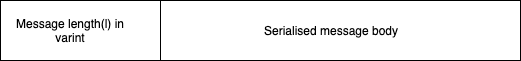
\includegraphics[width=11cm]{img/generic-message-encoding.png}
  \caption{generic message envelope encoding} 
  \label{img:generic_message_encoding}
\end{figure}

Maximum length(\textit{l}) of a generic message envelope or the maximum size of a message in Centrifuge network is currently limited to 32MB.






\section{User Mintable Non-Fungible Tokens}
\label{sec:nft}
To allow for the integration of Centrifuge documents into other applications built on Ethereum, Centrifuge implements a smart contract library for minting non-fungible tokens (NFTs as specificed by ERC721). NFTs are a widely adopted standard to create objects that have trackable and unique ownership. Centrifuge extends this standard with methods that allow users to mint these NFTs based on the private off-chain data in a document. When invoking the mint method on an $\mathsf{NFTRegistry}$, a set of fields of the document have to be revealed as merkle proofs, using the precise-proofs library. This information can then be stored in the token registry. We call this data metadata. Semantically, an NFT can have any kind of meaning for the application using it. The protocol itself does not impose any meaning to the tokens but merely provides a verifiable way to mint tokens for specific document states. The contract library provides the helpers to ensure that for one document only one token is minted in an NFT registry, that certain access rights are granted, and that the document is of a valid structure. Centrifuge, however, does define and deploy a number of registries that have a semantic meaning, most notably the Payment Obligation NFT. %TODO Reference 

\subsection{Non-Fungible Token Contract}
An NFT is a unique token that is always owned by one entity (an Ethereum account or contract). A token registry contract is a smart contract that manages a set of tokens.
\begin{description}
\item{\textbf{Registry Contract}} is a smart contract implementing the logic to create and transfer tokens. We define it as $\mathsf{NFTRegistry}$
\item{\textbf{Registry Contract Address}} the Ethereum address of the  $\mathsf{NFTRegistry}$ 
\item{\textbf{Token Identifier}} a $\mathbb{B}_{32}$ value defines the unique identifier of the token in the given registry contract, formally $T_{\mathtt{id}}$
\item{\textbf{Owner}} a $\mathbb{B}_{20}$ value of the Ethereum account or contract that is the owner of the token, formally $T_{\mathtt{owner}}$
\item{\textbf{Anchor}} a $\mathbb{B}_{32}$ value of the document identifier that the token is minted for, formally $T_{\mathtt{anchor}}$  %TODO: Ref to anchor
\item{\textbf{Metadata}} additional data that is supplied when the token is minted, formally $T_{\mathtt{meta-data}}$
\item{\textbf{Constraints}} defines an array of constraints for specific document fields. It  defines required values for the concrete document fields. For example, the an invoice status field to be \textit{unpaid} formally $T_{\mathtt{constraints}}$
\end{description}
\subsection{Minting a Token}
NFTs are created by calling the \texttt{mint} method of an NFT contract. The \texttt{mint} method requires the submission of a set of Merkle proofs for specific fields of the document for which the token has been minted. E.g. proofs for the invoice due date, amount, and currency in order to mint a token representing a payment obligation NFT. The Merkle proofs are validated by the NFT contract and checked against the document root provided by the Centrifuge.
\textit{AnchorRepository}. Any user who can produce valid proofs can mint the NFT. Together with the Merkle proof a second contract call is sometimes required. For example to proof a signature the Merkle proof verifies that a signature is part of a the document and a second call to an identity contract call would verify the signature itself.
\\The mint method can be defined as:\\
\begin{equation}
    \textsf{mint}(T_{\texttt{owner}}, T_{\texttt{id}},T_{\mathtt{meta-data}},d_{\mathtt{current}},d_{\mathtt{next}}, (P_{0},\dots, P_{n})) \xrightarrow[]{\text{ETH}} \mathsf{Identity} \xrightarrow[]{\text{ETH}}  \mathsf{NFTRegistry}
    %M_{\texttt{proof}}(R_{\texttt{doc-root}})
\end{equation}\\
A node doesn't call the mint method of the NFT Registry directly. The proxy functionality of the identity contract is used together with an action key $k_\mathtt{action}$ \textsf{mint} stored inside the node.\\\\
The mint method requires a set of proofs $(P_{[0]},...,P_{[n]})$ to perform the merkle proofs.
\begin{equation}
\begin{split}
P = (P_{\mathtt{field}},P_{\mathtt{sibling-hashes}}) \qquad
P_{\mathtt{field}} \in F \quad \And \quad P_{\mathtt{sibling-hashes}} \in \mathbb{B}_{32}^n 
\end{split}
\end{equation}

\subsubsection{Getting the Anchors}
The mint method needs the anchor for $d_{\mathtt{current}}$ to perform the merkle proofs based on the document root.
\begin{equation}
\begin{split}
{\scriptscriptstyle \mathsf{NFTRegistry}}  {\scriptscriptstyle &\xleftarrow[]{\text{ETH}}}  {\scriptscriptstyle \mathsf{AnchorRepository}} \\
{A_{\texttt{anchor-current}} &\xleftarrow[]{\text{ETH}} \textsf{getCommit}(d_{\mathtt{current}})}
\end{split}
\end{equation}
\textsf{NFTRegistry} calls the \textsf{AnchorRepository} to receive the document root (anchor) of the document. 

\subsubsection{Merkle Proof}
A Merkle proof can be seen as a function which proves if a provided field $P_\mathtt{field}$ is part of document. By calling the NFT mint method the value of these fields is revealed to the public. 
\begin{equation}
\begin{split}
v = \mathcal{M}_{\texttt{proof}}(A_{\texttt{anchor-current}},P_\mathtt{field},P_\mathtt{sibling-hashes}) \\
v \in \{0;1\}
\end{split}
\end{equation}
The $P_\mathtt{field}$  could be any field of the core document $d_C$ or the schema field $d_S$. The required $P_\mathtt{sibling-hashes}$ can be generated with the precise proofs library inside the node and contains the siblings of the field in each layer of the merkle tree.  
\subsubsection{Individual Field Merkle Proof}
Every NFT registry defines a set of mandatory fields on the document which need to be revealed. The mandatory fields depend on the purpose of the NFT and are defined by the initialization of the smart contract.
\begin{equation}
\begin{split}
\mathcal{M}_{\texttt{proof}}(A_{\texttt{anchor-current}} ,P_{[i]\mathtt{field}},P_{[i]\mathtt{sibling-hashes}}) = 1
\end{split}
\end{equation}
Every mandatory field requires a proof to verify that it is part of the document. Some mandatory fields could require the $P_{[i]\mathtt{field.value}}$ to have a concrete value.
\begin{equation}
    P_{[i]\mathtt{field.value}} = T_{\mathtt{constraints}[\mathtt{field.name}]}
\end{equation}
The required values are defined in the contract itself and are formally noted as $T_{\mathtt{constraints}}$. An example could be the status field of an invoice needs to be \textit{unpaid} for a specific NFT registry. It is possible to implement more complex conditions in a registry contract. Like the value of a fields needs to equal one out of $n$ pre defined values. 
\subsubsection{Latest Document}
A document can have multiple versions. It should be only possible to mint an NFT out of the latest document version. The $d_{\mathtt{next}}$ defines the anchor id of the next version. The mint method receives $d_{\mathtt{next}}$ as a parameter and can fetch the $A_{\texttt{anchor-next}}$ from the anchor registry.
\begin{equation}
\begin{split}
\mathsf{NFTRegistry} &\xleftarrow[]{\text{ETH}}  \mathsf{AnchorRepository} \\
A_{\texttt{anchor-next}} &\xleftarrow[]{\text{ETH}} \textsf{getCommit}(d_{\mathtt{next}})
\end{split}
\end{equation}
If $A_{\mathtt{anchor-next}}$ is not existing in the anchor registry and the $d_{\mathtt{next}}$ is part of document root.
\begin{equation}
\begin{split}
A_{\texttt{anchor-next}}  = \emptyset \quad \land \quad
\mathcal{M}_{\texttt{proof}}(A_{\texttt{anchor-current}} ,P_{[\mathtt{next}]\mathtt{field}}, &P_{[\mathtt{next}]\mathtt{sibling-hashes}})  = 1
\end{split}
\end{equation}
The $A_{\mathtt{anchor-current}}$ is the document root and $d_\mathtt{current}$ is the id of the latest document version.
\subsubsection{Verify an identity}
A NFT registry should be called by an identity contract. It makes it easier to verify signatures later on. Only identity contracts created by the Centrifuge Identity factory are accepted. Every provided collaborator DID can be verified by checking if the factory contract created the collaborator's identity contract. First, it needs to be verified that the collaborators $DID$ is part of the document.
\begin{equation}
\mathtt{msg.sender} = I_{\mathtt{DID}}
\end{equation}
For the document collaborator who wants to mint the document the Ethereum \texttt{msg.sender} is equal to their $DID$. In a second step the identity factory is called to verify if it an identity contract.
\begin{equation}
\begin{split}
\mathcal{M}_{\texttt{proof}}(A_{\texttt{anchor-current}} ,P_{[\mathtt{collaborator.did}]\mathtt{field}}, &P_{[\mathtt{collaborator.did}]\mathtt{sibling-hashes}})  = 1 \\
\mathsf{NFTRegistry} &\xleftarrow[]{\text{ETH}}  \mathsf{IdentityFactory} \\
v &\xleftarrow[]{\text{ETH}} \textsf{createdIdentity}(\mathtt{P_{[\mathtt{collaborator.did}]}}) \\
v & = 1 \\
\end{split}
\end{equation}

\subsubsection{Verify a Signature}
Providing a signature of a collaborator as part of a NFT minting ensures that the collaborator agreed on the document state. Agreement means a document rule $d_rules$ or a schema validation was not violated. For verifying a signature of the document signing root $R_\mathtt{signing}$ five steps are required.
\textbf{Signature part of document} \\
First a merkle proof verifies that a provided signature is part of the document.
\begin{equation}
\begin{split}
\mathcal{M}_{\texttt{proof}}(A_{\texttt{anchor-current}} ,P_{[\mathtt{signature}]\mathtt{field}},P_{[\mathtt{signature}]\mathtt{sibling-hashes}}) = 1 \\
\end{split}
\end{equation}
\textbf{Collaborator part of the document} \\
In a second merkle proof the DID of the collaborator who signed the document needs to be part of the document collaborators.
\begin{equation}
\begin{split}
\mathcal{M}_{\texttt{proof}}(A_{\texttt{anchor-current}} ,P_{[\mathtt{collaborator.did}]\mathtt{field}},P_{[\mathtt{collaborator.did}]\mathtt{sibling-hashes}}) = 1 \\
\end{split}
\end{equation}
\textbf{Signing root part of the document} \\
A third merkle proof verifies that the siging root $R_\mathtt{signing}$ is part of the document.
\begin{equation}
\begin{split}
\mathcal{M}_{\texttt{proof}}(A_{\texttt{anchor-current}} ,P_{[\mathtt{signing-root}]\mathtt{field}},P_{[\mathtt{signing-root}]\mathtt{sibling-hashes}}) = 1 \\
\end{split}
\end{equation}
\textbf{Collaborator identity verification} \\
The DID of the collaborator needs to be an ERC725 identity contract created by the Identity factory.
\begin{equation}
\begin{split}
\mathsf{NFTRegistry} &\xleftarrow[]{\text{ETH}}  \mathsf{IdentityFactory} \\
v &\xleftarrow[]{\text{ETH}} \textsf{createdIdentity}(\mathtt{msg.sender}) \\
v & = 1
\end{split}
\end{equation}
\textbf{Verify the signature of the Collaborator} \\
If the DID of the collaborator is a ERC725 identity contract. The NFTRegistry can call the signature verification method on it.
\begin{equation}
\begin{split}
\mathsf{NFTRegistry} &\xleftarrow[]{\text{ETH}}  \mathsf{Identity} \\
K_{\texttt{purpose}} & = \mathtt{sha256("CENTRIFUGE@SIGNING"))} \\
v &\xleftarrow[]{\text{ETH}} \textsf{isSignedWithPurpose}(P_{[\mathtt{signing-root}]\mathtt{field}},P_{[\mathtt{signature}]\mathtt{field}},K_{\texttt{purpose}}))\\
v & = 1
\end{split}
\end{equation}
\\
If the signature was signed with the purpose key for signing the signature is accepted by the mint method.

\subsubsection{Uniqueness Enforcement}
A document can have multiple different NFT's for different purposes. Nevertheless it should be not possible to mint the exact same NFT twice for the same document in the same registry. For example an NFT which could represent a payment obligation of an invoice should be only allowed to be minted once. For enforce the requirement the NFT id $T_{id}$ together with the NFT registry address needs to be part of the document. 
\begin{equation}
\begin{split}
N & = (N_{\mathtt{registry-id}}, N_{\mathtt{token-id}}) \\
N_{\mathtt{registry-id}} \in \mathbb{B}_{32}  \quad &\land \quad N_{\mathtt{token-id}} \in \mathbb{B}_{32}  \\
d_{\mathtt{nfts}}& = (N_{[0]},...,N_{[n]})
\end{split}
\end{equation}
A collaborator who wants to mint an NFT first needs to create a new document version $d'$.
\begin{equation}
\begin{split}
N'_{\mathtt{token-id}} & = \texttt{RAND(32)}\\
N'_{\mathtt{registry-id}} & = T_{\mathtt{registry-address}} \quad \| \quad \mathbb{B}_{12} \\
N'  & = (N'_{\mathtt{registry-id}},N'_{\mathtt{token-id}}) \\
d' & = d \\
d'_{\mathtt{nfts}} & = \texttt{append}(d_{\mathtt{nfts}},N')
\end{split}
\end{equation}
The new document version $d'$ needs to include the token id $T_{\mathtt{id}}$ which can be randomly chosen by
the user and the registry address itself. In Protobuf definition of the document $d_{\mathtt{nfts}}$ is implemented as a map where the key is 32 bytes including the 20 bytes of the Ethereum registry address and 12 bytes of zeros in the end. The user needs to request the signatures of the collaborators and commit the new document version as described in a previous chapter. (See chapter \ref{sec:consensus})
\begin{equation}
\begin{split}
\mathcal{M}_{\texttt{proof}}(A_{\texttt{anchor-current}} ,P_{[\mathtt{nfts]{[registry-address]}}\mathtt{field}},P_{[\mathtt{nfts]{[registry-address]}}\mathtt{sibling-hashes}}) &= 1 \\
P_{[\mathtt{nfts]{[registry-address]}}\mathtt{field.value}} &= T_{\mathtt{id}}
\end{split}
\end{equation}
Inside the mint method a merkle proofs verifies that the provided $T_{id}$ is part of the document. A collaborator would not sign a new document version $d'$ if the current one already includes a token id for the same NFT registry. Without the signatures of the collaborators it is not possible to mint a token for the same registry twice.


\subsection{Token Methods}
The ERC721 standard defines the interface for a NFT registry.
\subsubsection{Transfer}
The token smart contract has a function to get the owner of a token by the token identifier. This method is compliant with the ERC721 standard

\begin{equation}
 T_{\mathtt{owner}} \xleftarrow[]{\text{ETH}} \mathsf{ownerOf}(T_{\texttt{id}})
\end{equation}
A token can be transferred by the current owner to a different owner:

\begin{equation}
\mathsf{transferTo}(T_{\texttt{id}},T_{\texttt{owner}},T_{\texttt{new-owner}}) \xrightarrow[]{\text{ETH}}  \mathsf{NFTRegistry}
\end{equation}
\subsubsection{Metadata}
Metadata 
 

\subsection{Document Access}
Over the life time of an NFT it can be transfered to different users and companies. A person or a user who owns an NFT has the option to request read access to the document which belongs to the NFT. The token owner needs to have a node and a DID. It is not required that the owner is in the list of document collaborators $d_{\mathtt{collaborators}}$.
\begin{equation}
    \begin{split}
            (\mathtt{DID_{sender}},T_{\mathtt{id}},T_{\mathtt{registry-address}},d_{\mathtt{id}})& \xleftarrow[]{\text{P2P}}  \mathsf{receiveDocumentRequest}(\mathtt{DID_{sender}}) \\
            T_{\mathtt{owner}}  & \xleftarrow[]{\text{ETH}} \mathsf{ownerOf}(T_{\texttt{id}}) \\
               d    &= \mathsf{loadLatestVersion}({d}_{\mathtt{id}}) \\
    \end{split}
\end{equation}
If the following condition is true the $\mathtt{DID_{sender}}$ is a NFT owner of the document.
\begin{equation}
    \begin{split}
     d_{\mathtt{nfts[T_{registry-address}]}} = T_{\mathtt{id}} \quad \land \quad T_{\mathtt{owner}} = \mathtt{DID_{sender}}
    \end{split}
\end{equation}
The provided token id $T_{\mathtt{id}}$ needs to be part of the document and the NFT owner in the registry needs to be the $\mathtt{DID_{sender}}$. If both requirements are fullfilled the document will be send.
\begin{equation}
      \mathsf{send}(d) \xrightarrow[]{\text{P2P}} \mathtt{DID_{sender}}
\end{equation}



\section{Revisions}
\label{sec:revisions}
This document is a working document that will be updated as the Centrifuge Protocol evolves. It is hosted at \url{https://github.com/centrifuge/protocol}. Additions and changes are welcome. 
\subsection{Notable Revisions}
\begin{enumerate}
    \item 17.05.2019 (\texttt[caf6e80]): First public release of paper, covers Centrifuge Beta launch
    \item 17.03.2019 (\texttt{8c4357b}): First draft version
\end{enumerate}



%---------------------------------------------------
%----- Bibliography
%---------------------------------------------------
\phantomsection
\addcontentsline{toc}{chapter}{Literature}
\bibliographystyle{plain}
\bibliography{references.bib}



%\printacronyms[include-classes=nomencl,name=Nomenclature]
%\printacronyms[include-classes=abbrev,name=Abbreviations]
\begin{comment}
\section{Appendix}

\subsection{ERC725 Contract}\label{app:identity_contract}

% Question: I might replace it with a normal table. We maybe should put it in the appendix, anyway.
% Just trying things out
\lstdefinelanguage{solidity}{
  keywords={contract,break, case, catch, continue, debugger, default, delete, do, else, finally, for, function, if, in, instanceof, new, return, switch, this, throw, try, typeof, var, void, while, with, event},
  keywordstyle=\color{blue}\bfseries,
  ndkeywords={uint256,bytes32}
  ndkeywordstyle=\color{blue}\bfseries,
  identifierstyle=\color{black},
  morecomment=[l]{//},
  morecomment=[s]{/*}{*/},
  morestring=[b]',
  morestring=[b]",
  sensitive=true
}
\begin{lstlisting}[language=solidity]
pragma solidity ^0.4.18;

contract ERC725 {

    uint256 constant MANAGEMENT_KEY = 1;
    uint256 constant ACTION_KEY = 2;
    uint256 constant CLAIM_SIGNER_KEY = 3;
    uint256 constant ENCRYPTION_KEY = 4;

    event KeyAdded(bytes32 indexed key, uint256 indexed purpose, uint256 indexed keyType);
    event KeyRemoved(bytes32 indexed key, uint256 indexed purpose, uint256 indexed keyType);
    event ExecutionRequested(uint256 indexed executionId, address indexed to, uint256 indexed value, bytes data);
    event Executed(uint256 indexed executionId, address indexed to, uint256 indexed value, bytes data);
    event Approved(uint256 indexed executionId, bool approved);

    struct Key {
        uint256 purpose; //e.g., MANAGEMENT_KEY = 1, ACTION_KEY = 2, etc.
        uint256 keyType; // e.g. 1 = ECDSA, 2 = RSA, etc.
        bytes32 key;
    }

    function getKey(bytes32 _key) public constant returns(uint256[] purposes, uint256 keyType, bytes32 key);
    function keyHasPurpose(bytes32 _key, uint256 purpose) constant returns(bool exists);
    function getKeysByPurpose(uint256 _purpose) public constant returns(bytes32[] keys);
    function addKey(bytes32 _key, uint256 _purpose, uint256 _keyType) public returns (bool success);
    function execute(address _to, uint256 _value, bytes _data) public returns (uint256 executionId);
    function approve(uint256 _id, bool _approve) public returns (bool success);
    }
\end{lstlisting}
\end{comment}

\end{document}

